%%
%% Objective 2 — polyglot bug localization.
%% Drafted in the Elsevier CAS double-column format (JSS) reused from
%% Objective 1; to be converted to ACM acmart (TOSEM) later.
%%
%% Markers used while drafting (all render in colour; remove before submission):
%%   \pending{...}     a result that needs the full runs
%%   \missingcite{...} a citation still to be found / verified
%%   \gap{...}         something the draft shows is missing in the study itself
%%

\documentclass[a4paper,fleqn]{cas-dc}

\usepackage[authoryear]{natbib}
\usepackage{booktabs}
\usepackage{multirow}
\usepackage{xspace}
\usepackage{xcolor}
\usepackage{enumitem}
\usepackage{tikz}
\usepackage[most]{tcolorbox}
\usepackage{adjustbox}
\usepackage[expansion=false]{microtype}
\tcbset{colback=gray!6,colframe=gray!60,fonttitle=\bfseries\small,fontupper=\small,left=4pt,right=4pt,top=2pt,bottom=2pt}
\usetikzlibrary{arrows.meta,positioning,fit,backgrounds}

\newcommand{\pending}[1]{\textcolor{red!70!black}{[PENDING: #1]}}
\newcommand{\missingcite}[1]{\textcolor{orange!80!black}{[CITE: #1]}}
\newcommand{\gap}[1]{\textcolor{blue!70!black}{[GAP: #1]}}
\newcommand{\mono}{Mono-fix\xspace}
\newcommand{\poly}{Poly-fix\xspace}

\begin{document}
\let\WriteBookmarks\relax
\def\floatpagepagefraction{1}
\def\textpagefraction{.001}

\shorttitle{Mono-fix or Poly-fix? Bug fixes beyond the main language}
\shortauthors{Rao and Chimalakonda}

\title[]{Mono-fix or Poly-fix? Bug Fixes Beyond the Main Language and Their Effect on Bug Localization}

\author[1]{A Eashaan Rao}[orcid=https://orcid.org/0000-0001-8499-7538]
\cormark[1]
\ead{cs21d002@iittp.ac.in}

\author[1]{Sridhar Chimalakonda}[orcid=https://orcid.org/0000-0003-0818-8178]
\ead{ch@iittp.ac.in}

\affiliation[1]{organization={Indian Institute of Technology Tirupati},
            city={Tirupati},
            postcode={517619},
            state={Andhra Pradesh},
            country={India}}

\cortext[1]{Corresponding author}

%% ===================================================================
%% ABSTRACT
%% ===================================================================
\begin{abstract}
Bug localization ranks a project's files by how likely each is to need a
change for a bug report. Its benchmarks and techniques assume that a fix
changes source files of the project's main language. We call a fix
\emph{Mono-fix} if the files it changes belong to one language and
\emph{Poly-fix} if they belong to several, for example a Java class and a YAML
configuration file. Among 3{,}594 bugs from six Java and Python projects of
BeetleBox, 8.2--27.4\% of the fixes are Poly-fix, depending on
which files count, and about
two-fifths of the files these fixes change cannot be read by a Java or Python
parser. Of five techniques, evaluated on time-ordered splits, BM25 and BLAZE
read every file; FLIM, the agent LocAgent and the ranker
SweRank (Python projects only) see only the files their parser accepts. FLIM
ranks the fixed files of Poly-fix bugs worse than those of Mono-fix bugs
(mean average precision 0.25 against 0.37); for BM25 and BLAZE the drop is
smaller and not significant. All three parser-dependent techniques lead BM25
on Mono-fix bugs and lose that lead on Poly-fix bugs. Mean reciprocal rank and Top-$k$
accuracy, which reward only the first fixed file found, weaken these effects
and show no reversal. For SweRank, diagnostic variants point to reach:
given every text file, it ranks the non-Python files at least as well as
BM25, and its Poly-fix penalty falls by about three quarters, from 0.17 to
0.04; the non-Python files, not the test files, account for the reduction.
\end{abstract}

\begin{keywords}
Bug Localization \sep Polyglot Software \sep Multi-Language Systems \sep
Empirical Study \sep Mining Software Repositories
\end{keywords}

\maketitle

%% ===================================================================
%% 1 INTRODUCTION
%% ===================================================================
\section{Introduction}\label{sec:intro}

Bug localization takes a bug report and returns a ranked list of the files of a
project, ordered by how likely each file is to need a change
\citep{zhou2012should,lee2018bench4bl}. Information-retrieval-based (IR-based)
techniques compute this ranking from the text of the report and the content of
the files. They range from classical lexical retrieval
\citep{robertson2009probabilistic,zhou2012should} to learned rankers that use
pre-trained code models \citep{liang2022modeling,chakraborty2025blaze} and,
most recently, to techniques built on large language models (LLMs): agents
that search a repository with tools
\citep{yang2024sweagent,xia2024agentless,chen2025locagent} and rankers that
reorder the code an embedding model retrieves \citep{reddy2025swerank}.

The evaluation of these techniques rests on an assumption that is rarely
stated: that the files a fix changes are source files of the project's main
language. Standard benchmarks are built this way; Bench4BL indexes and scores
Java files only \citep{lee2018bench4bl}. The dataset-quality literature has
asked which changed files should count as ground truth, but its concern is
the opposite case, files that a fix changes without being buggy
\citep{kochhar2014potential}; whether the files a fix needs can lie outside
the main language has not been examined. Real fixes are not always contained
in that set. In localstack, the fix for issue~8030 (``CreateMultipartUpload
should return InitiateMultipartUploadResult element'') changes three Python
files and \texttt{localstack/aws/spec-patches.json}, a JSON patch to the AWS
API specification that the serializer reads.

When a fix crosses file types, two different things can go wrong for a
localization technique. A technique that parses source code into a structured
representation---functions, abstract syntax trees, code graphs---may have no
parser for the file and therefore cannot represent it at all. Or the technique
can read the file but ranks it poorly, because its vocabulary and structure
differ from the source files the technique was trained on. We call the first
a limit of \emph{reach} and the second a limit of \emph{representation}.
Ranking metrics reported over a whole benchmark do not separate them.

The distinction matters for how the field reads its own progress. Classical
retrieval treats every file as a bag of tokens and can process any text file.
The techniques that cannot are those that need a parser to represent a
file---we call them \emph{parser-dependent}---and parsing structure is what
distinguishes them from classical baselines. If parser-dependent techniques
lose ground on fixes that cross file types, part of their reported advantage
over classical retrieval may hold only on the portion of the task they can
read. This paper reports an exploratory study of that question. The unit of
analysis is the fix, classified from the files of the fix commit
(Section~\ref{sec:definitions}). We ask five research questions:

\begin{description}[leftmargin=0pt,itemsep=2pt]
\item[RQ1 (Prevalence).] What proportion of fixes are Poly-fix, and to which
  file types do the additional files belong?
\item[RQ2 (Reach).] How much of each Poly-fix fix can each technique
  represent at all?
\item[RQ3 (Performance by fix type).] How does each technique's localization
  performance differ between Mono-fix and Poly-fix bugs of the same project?
\item[RQ4 (Classical baseline).] On Poly-fix bugs, does classical retrieval
  match or exceed the techniques that depend on a parser?
\item[RQ5 (Reach or representation).] When a parser-dependent technique is
  given the files it cannot represent, does its Poly-fix penalty shrink, and
  which of the added files cause the change?
\end{description}

\noindent In brief, Poly-fix fixes are common, though how common depends on
which files count, and a parser-dependent technique cannot read about
two-fifths of the files they change (RQ1, RQ2). Every parser-dependent
technique we ran ranks the fixed files of Poly-fix bugs worse than those of
Mono-fix bugs, while for BM25 and BLAZE the drop is smaller and not
significant (RQ3). The parser-dependent techniques' lead over BM25 on Mono-fix
bugs is lost on Poly-fix bugs; mean reciprocal rank and Top-$k$ accuracy
weaken this and show no reversal (RQ4). When SweRank is given every text file,
its penalty falls by about three quarters, and the non-Python files account
for the reduction (RQ5, exploratory).

Part of the penalty follows by construction: a technique that cannot see a
fixed file cannot rank it. What does not follow by construction is what this
paper contributes: how often fixes contain such files, whether the techniques
that can see them rank them well, how large the penalty is next to the
advantage parser-dependent techniques show elsewhere, and which metrics reveal
it. The contributions are:
\begin{itemize}[itemsep=1pt]
\item a classification of bug fixes by the languages of the files they change
  (Mono-fix / Poly-fix), with explicit rules for which files count, applied to
  3{,}594 bugs, and the prevalence it yields under each rule (RQ1);
\item a per-file account of which fixed files each technique can read, which
  separates a technique that cannot see a file from one that sees it but ranks
  it poorly (RQ2, RQ3, RQ5);
\item a comparison of five techniques that differ in what they can read, on a
  time-ordered split of each project, with every file ranked and one evaluator
  for all techniques (RQ3, RQ4);
\item the classification, per-file parse status, score files and scripts
  \pending{replication package DOI}.
\end{itemize}

\noindent Section~\ref{sec:background} positions the study,
Section~\ref{sec:design} describes its design, Section~\ref{sec:results} the
results, Section~\ref{sec:discussion} their implications and
Section~\ref{sec:threats} the threats to validity. Appendices~A--G
(supplementary material) give the supporting tables and analyses.

%% ===================================================================
%% 2 BACKGROUND AND RELATED WORK
%% ===================================================================
\section{Background and Related Work}\label{sec:background}

\subsection{IR-based bug localization techniques}

We group techniques by what their architecture can read, the property this
study varies. \emph{Classical retrieval} scores report and file as bags of
terms with a lexical model such as VSM or BM25
\citep{robertson2009probabilistic}; BugLocator added similar-report history
\citep{zhou2012should}. Any text file can be indexed. \emph{Learned rankers}
learn a relevance function from past fixes: Ye et al.\ combined lexical,
history and structure features with learning to rank \citep{ye2014learning},
and Fejzer et al.\ adapt the feature weights per project
\citep{fejzer2022tracking}. FLIM splits each file into functions with a
language parser, fine-tunes CodeBERT \citep{feng2020codebert} on
(report, function) pairs and fuses the similarities with IR features in a
learning-to-rank model \citep{liang2022modeling}; BL-GAN encodes files as AST
graphs \citep{zhu2022bl}. BLAZE fine-tunes a language-agnostic code embedding
model on report--chunk pairs; a tree-sitter parser only chooses chunk
boundaries, so any text can be embedded \citep{chakraborty2025blaze}.

\emph{LLM-based techniques} use a large language model as an agent or as a
ranker. SWE-agent exposes shell-like commands \citep{yang2024sweagent},
Agentless runs a fixed sequence of prompts over a repository skeleton
\citep{xia2024agentless}, and AutoCodeRover \citep{zhang2024autocoderover} and
LocAgent \citep{chen2025locagent} search code entities. LocAgent's tools
navigate a graph of directories, files, classes and functions built by
parsing Python source, so they can only reach what the parser produced.
SweRank \citep{reddy2025swerank} retrieves the 100 functions most similar to
the report with an embedding model and reorders them with a fine-tuned LLM;
both stages work on functions parsed from non-test Python files. SweRank+
extends it to ten languages \citep{reddy2025sweranplus}, but its models and
code are not public.

\subsection{Fixes, ground truth and multi-language software}

Prior characterisations describe a fix by how much it changes and where:
Nashid et al.\ classify multi-hunk patches by spatial dispersion and show that
LLM repair succeeds less often as dispersion grows \citep{nashid2025multihunk},
and an agent-based localization study extends the Bench4BL ground truth with
the methods each fix modified \citep{samir2026cognigent}. We classify fixes by
\emph{composition}---the file types they contain. Work on dataset quality asks
whether the ground truth is correct: misclassified reports
\citep{herzig2013its}, tangled fix commits \citep{herzig2013impact} and their
effect on measured performance \citep{kochhar2014potential}. It concerns files
that should \emph{not} be in the ground truth; we study files that fixes
contain and that an evaluation may not reach. BLAZE introduced BeetleBox, a
dataset spanning five languages \citep{chakraborty2025blaze}, but its unit is
still a fix within a project of one language. xLoc localizes bugs caused by
interactions between Python and C \citep{yang2024xloc}: a bug caused by a
language boundary, not a fix that crosses one. Most open-source projects use
several languages \citep{mayer2015empirical}, multi-language use has been
associated with defect-proneness \citep{kochhar2016large}, and regression test
selection tools are unsafe on polyglot projects because they miss
inter-language dependencies \citep{celik2017rtslinux}, the closest precedent
of a monolingual tool applied to a polyglot artefact.
Table~\ref{tab:positioning} (Appendix~\ref{app:related}) summarises what each
line of work provides and what this study adds.

%% ===================================================================
%% 3 STUDY DESIGN
%% ===================================================================
\section{Study Design}\label{sec:design}

The study is exploratory: the research questions are descriptive, a
statistical test is run only where a specific comparison calls for one, and a
null result at any step is reported as a result. Figure~\ref{fig:design}
summarises the pipeline.

\begin{figure*}[pos=t]
\centering
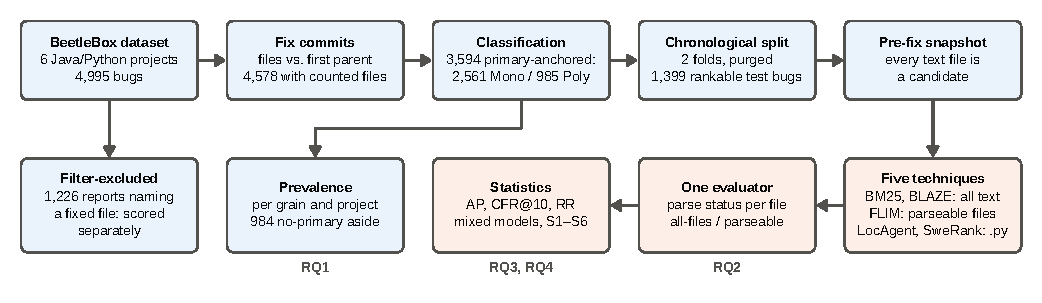
\includegraphics[width=\textwidth]{figures/study_design.pdf}
\caption{Study design. Blue: data preparation; orange: evaluation. Every technique scores every candidate file of the pre-fix snapshot; one evaluator computes all metrics. The diagnostic variants of RQ5 (ours, not proposed techniques) were added after RQ3 and RQ4.}
\label{fig:design}
\end{figure*}

\subsection{Definitions}\label{sec:definitions}

Table~\ref{tab:terms} lists the terms used throughout. The \emph{fix} of a bug
is the commit the dataset links to it; its \emph{fix files} are the files the
commit adds, modifies, deletes or renames relative to its first parent.
Documentation, changelog fragments, lock files, generated and vendored files,
CI and tooling configuration, binaries and deleted files are excluded by
\emph{boundary rules} (Section~\ref{sec:classification}); the remaining fix
files are \emph{counted}. A file's language is decided from its extension, or
its name (e.g.\ \texttt{Dockerfile}).

The \emph{primary language} of a project is Java or Python; a
\emph{secondary-language file} is a counted file in any other language. A bug
is \emph{Mono-fix} if all its counted fix files belong to one language, and
\emph{Poly-fix} if they belong to two or more. Which secondary languages count
is the \emph{grain}. The \emph{broad} grain, used throughout, counts any
language that has a formal grammar and whose files are read by programs
(YAML, JSON, XML, Shell, Groovy, \ldots); the \emph{data-format} grain counts
only YAML, JSON, XML and SQL, and the \emph{strict} grain only programming
languages. A bug is \emph{primary-anchored} if at least one counted fix file is
in the primary language, so every such bug has a target a Java or Python
parser can read; the Mono-fix/Poly-fix comparison uses these bugs only. A bug
with counted fix files but none in the primary language is \emph{no-primary}
and analysed separately.

A secondary-language fix file is a \emph{test asset} if it lies under a test
path: recorded snapshots, expected outputs, test playbooks, REST test
specifications. Changing it changes what the tests expect, not what the
software does. A Poly-fix bug is \emph{behaviour-bearing} if at least one
secondary file is not a test asset (configuration, schema, build script, API
specification, source in another language) and \emph{test-asset-only}
otherwise; every Poly-fix result is reported for both sub-types. A file is
\emph{parseable} if the project-language parser accepts it (CPython's
\texttt{ast}; tree-sitter-java); a file of another language has status
\texttt{no\_parser}, a rejected one \texttt{parse\_error}. A fixed file is
\emph{reachable} if it exists before the fix. \emph{Classical retrieval} can
index any text file; a \emph{language-agnostic} technique embeds any text,
using a parser at most to cut chunks; a \emph{parser-dependent} technique can
represent a file only through a parser's output.

\begin{table}[t]
\caption{Key terms.}
\label{tab:terms}
\footnotesize
\begin{adjustbox}{max width=\linewidth}\begin{tabular}{p{3.0cm}p{5.0cm}}
\toprule
Term & Meaning \\
\midrule
Counted file & Fix file not excluded by a boundary rule \\
Primary language & Java or Python, the project's main language \\
Secondary-language file & Counted fix file in any other language \\
Mono-fix / Poly-fix bug & Counted fix files in one / several languages \\
Primary-anchored bug & Has a counted primary-language fix file; used in the main comparison \\
Filter-excluded bug & Report BeetleBox excluded because it names a fixed file; analysed separately \\
No-primary bug & Has counted fix files, none in the primary language \\
Behaviour-bearing Poly-fix & At least one secondary file is read by the running or built software \\
Test-asset-only Poly-fix & All secondary files are test assets \\
Parseable file & Accepted by the project-language parser \\
Reachable file & Exists before the fix (not added by it) \\
All-files / parseable view & Every file is a candidate / only parseable files are \\
FLIM-strict / FLIM-fallback & FLIM as published / FLIM with text windows for unparseable files (ours) \\
\bottomrule
\end{tabular}\end{adjustbox}
\end{table}

\subsection{Dataset and project selection}\label{sec:dataset}

We use BeetleBox \citep{chakraborty2025blaze}, the only public
bug-localization dataset we know of whose ground truth includes files of
several languages and file types. It has 13 Java and Python projects with at
least 100 bug reports, enough for a within-project comparison of the two
classes. Our compute budget for training and evaluating five techniques on
every project and fold allowed six projects, three per language
(Table~\ref{tab:dataset}). Among the eligible projects we chose ones in which
both classes would be populated, checked with a proxy: the share of fixes that
change files with more than one extension is 29--66\% in each of the six. Two
further projects pass this proxy (openrefine and posthog); the choice among
the qualifying projects was ours, not a rule, and the localization results
were not known when it was made. The selection is purposive and favours
projects rich in Poly-fix fixes (Section~\ref{sec:threats}).

Java and Python are the languages in which bug localization is evaluated: the
standard IR-based benchmarks are Java \citep{lee2018bench4bl,ye2014learning}
and those for LLM-based localizers Python \citep{jimenez2023swe}. The
parser-dependent techniques were also built for them---FLIM on Java,
LocAgent and SweRank on Python---so a failure is not an artefact of our
porting a parser. FLIM's design is language-independent apart from its parser
and one feature, so we run it on both languages; LocAgent and SweRank depend
on models trained on Python only.

For all 4{,}995 bugs of the six projects the fix commit was recovered;
3{,}594 (72.0\%) are primary-anchored, 417 change no counted file, and 984
change counted files but none in the primary language (no-primary; mostly the
TypeScript and Vue front-end of dolphinscheduler and configuration-only
fixes). When BeetleBox was built, reports that name a fixed file were removed
``to ensure the quality of the dataset'' \citep{chakraborty2025blaze}; for our
projects these are 1{,}226 reports, released separately. Because naming the
file is where lexical retrieval is strongest, these \emph{filter-excluded}
bugs and the no-primary bugs are analysed as separate groups
(Section~\ref{sec:removed}).

\subsection{Classification procedure}\label{sec:classification}

The ruleset was written before any bug was classified and frozen as version
0.2.0. Path rules are applied before the extension map: changelog fragments,
lock files, vendored and generated paths, CI configuration, developer tooling
and documentation are excluded; test files and test assets are kept and
tagged. A secondary language makes a fix Poly-fix only if (C1) it has a formal
grammar, (C2) the project's parser cannot read it, (C3) its files are read by
programs rather than by people, and (C4) its files are part of the dataset's
ground truth. 48 primary-anchored bugs are multi-language only through
languages that fail C1--C3 (e.g.\ plain-text templates) and are left out of
the class comparisons. The written protocol was checked on a stratified
sample of 50 bugs, annotated from the protocol alone without access to the
classifier: \pending{Two-person agreement (Cohen's $\kappa$) and its
resolution.} Appendix~\ref{app:design} gives the protocol details.

%% -------------------------------------------------------------------
\subsection{Techniques}\label{sec:techniques}

We evaluate one technique of each kind (Section~\ref{sec:definitions}) and two
parser-dependent techniques built on LLMs, an agent (LocAgent) and a
retrieve-and-rerank ranker (SweRank) (Table~\ref{tab:techniques}). FLIM and
BLAZE are re-implemented against their authors' released code, with every
departure listed in Appendix~\ref{app:design}; LocAgent and SweRank are run
from their released code and models. To avoid an advantage from BeetleBox
having been built alongside BLAZE, we train BLAZE from the public
CodeSage-small checkpoint and report it separately.

\begin{table*}[t]
\caption{Techniques. ``Reads'' is what the architecture can represent.}
\label{tab:techniques}
\small
\begin{adjustbox}{max width=\linewidth}\begin{tabular}{p{2.0cm}p{3.2cm}p{4.6cm}p{6.2cm}}
\toprule
Technique & Kind & Reads & Configuration \\
\midrule
BM25 & Classical retrieval & any text file, as tokens & bm25s 0.3.11, Lucene BM25, $k_1{=}1.2$, $b{=}0.75$; compound identifiers indexed whole and split; English stop words, no stemming; document = path + content \\
BLAZE \citep{chakraborty2025blaze} & Language-agnostic neural & any text file, as chunks & CodeSage-small \citep{zhang2024codesage}, full fine-tuning, residual adapters; dynamic chunking (tree-sitter); NT-Xent loss; $\le$15 epochs \\
FLIM \citep{liang2022modeling} & Parser-dependent & files the project-language parser accepts (functions; AST fields; import graph) & CodeBERT fine-tuned on (report, function) pairs, $\le$10 epochs; 4 semantic + 18 IR features; adaptive pointwise LTR \citep{fejzer2022tracking} \\
LocAgent \citep{chen2025locagent} & LLM agent over a parsed graph & Python files (graph from \texttt{ast}; BM25 index of non-test \texttt{.py} files) & Released code (\texttt{4935b55}), unmodified; the paper's fine-tuned Qwen2.5-Coder-7B (vLLM, bf16, 128k context); default sampling \\
SweRank \citep{reddy2025swerank} & LLM ranker over parsed functions & functions of non-test Python files & Released code (\texttt{d3df508}) and models; SweRankEmbed-Small retriever (137M) and SweRankLLM-Small reranker (7B); top 100 reranked in windows of 10, greedy decoding \\
\bottomrule
\end{tabular}\end{adjustbox}
\end{table*}

We do not adapt any technique to secondary languages: the object of study is
how existing techniques behave, and an adapted technique would be a new one.
FLIM-fallback and the RQ5 variants are diagnostic, labelled as ours, untuned
and reported separately. FLIM is parser-dependent by architecture: its
semantic features need the function list, and 13 of its 18 IR features use
parser output. LocAgent represents agents and SweRank, published four years
after FLIM, learned rankers. Neither LLM-based technique can index the Java
projects---both parse with Python's \texttt{ast} and were trained on Python
only, and the multilingual SweRank+ is not released---so both run on the
Python projects, and we report this as a feasibility result.
Appendix~\ref{app:design} explains why BL-GAN, TRANP-CNN and Agentless are
not run.

%% -------------------------------------------------------------------
\subsection{Evaluation setup}\label{sec:evaluation}

\paragraph{Split.} Within each project, bugs are ordered by report date; the
oldest 80\% form the training pool and the newest 20\% the test set (fold~1),
with the newest 10\% of the pool used for model selection. Bugs whose fix
landed after the next period started are purged, so no technique learns from a
fix that did not exist when the bugs it is evaluated on were reported. A
rolling-origin fold~2 trains on the oldest 60\% and tests on the next 20\%.
Over both folds, 1{,}399 Mono-fix and Poly-fix test bugs (981 and 418) have at
least one reachable ground-truth file.

\paragraph{Candidates and ground truth.} For each test bug, every technique
scores every text file of the pre-fix snapshot that the ruleset counts (the
universe R; 1{,}890 to 21{,}658 files per snapshot), with no pre-selection.
The ground truth is the bug's counted fix files at their pre-fix path, the
same files that define its class. It is the change set of the fix rather than
the fault location: a developer acting on a ranking must change every file of
the fix, and the standard benchmarks also derive their ground truth from the
changed files \citep{lee2018bench4bl,jimenez2023swe}. Because the change set
includes test snapshots and expected outputs, we give equal weight to two
fault-oriented views of every result: the ground truth without test files
(sensitivity S1) and the behaviour-bearing Poly-fix bugs.

\paragraph{Views.} Each technique is evaluated in the \emph{all-files} view,
where every file is a candidate, and in the \emph{parseable} view, where only
parseable files are and an unparseable ground-truth file counts as a miss.
For FLIM the parseable view is the published condition (FLIM-strict); in the
all-files view it represents unparseable files by line windows of their text
(FLIM-fallback, ours). Both come from one trained model.

\paragraph{Metrics.} Per bug we compute average precision (AP: the precision at
each hit, divided by the number of reachable ground-truth files; mean MAP),
the reciprocal rank of the first ground-truth file (RR; mean MRR), Top-$k$
and complete-fix recall@10 (CFR@10, the share of reachable ground-truth files
in the first 10). AP is the primary outcome, fixed before any full run: every
primary-anchored Poly-fix bug has a primary-language fix file, so a metric
that rewards only the first hit (RR, Top-$k$) cannot show whether a technique
reaches the rest of the fix. LocAgent returns at most ten files, so
comparisons that include it use AP@10 for every technique. LocAgent and
SweRank are run on the 790 test bugs of the three Python projects; files
SweRank cannot see share the last ranks (counting them as misses gives the
same class effect). SweRank's retriever alone is evaluated as a second
ranking. The filter-excluded and no-primary bugs of the test periods are
scored with the models trained on the primary-anchored bugs and never pooled
with them.

\paragraph{Diagnostic variants (RQ5).} A \emph{hybrid} ranks the files a
technique can represent by its own ranking and every other file by BM25,
merged by reciprocal rank fusion ($k{=}60$; \citealp{cormack2009rrf}). A
\emph{co-change} variant ranks the other files instead by how often they
changed, before the report, together with the technique's top five files
\citep{zimmermann2004mining}. \emph{SweRank on all text files} adds every
other candidate file to SweRank's corpus as 50-line chunks (at most 40 per
file) and runs retriever and reranker unchanged; partial corpora add only the
non-Python files, only the Python test files, or all files with at most 10
chunks. None is tuned. The variants, and RQ5 itself, were added after the
results of RQ3 and RQ4 were known, so RQ5 is exploratory;
Appendix~\ref{app:design} gives the implementation.

\paragraph{Training.} Hyper-parameters come from the authors' code except the
learning rate, chosen by validation MAP over a small grid around the published
values (Appendix~\ref{app:design}). Each neural technique is run with seed 13
on every project and fold and with two further seeds on fold~1 of three
projects; per-bug metrics are averaged over seeds.

%% -------------------------------------------------------------------
\subsection{Analysis}\label{sec:analysis}

RQ1 reports the share of primary-anchored bugs that are Poly-fix per grain and
project; RQ2 the share of ground-truth files each technique can represent,
from the parse status of every file. For RQ3 we compare per-bug AP between
Mono-fix and Poly-fix bugs within each project (Mann--Whitney U,
\citealp{mann1947test}; Cliff's $\delta$, \citealp{cliff1993dominance}) and
across projects with a linear mixed model
$\mathrm{AP} \sim \mathrm{class} + n_{\mathrm{gt}} + \log n_{\mathrm{cand}} +
\ell_{\mathrm{report}} + \mathrm{fold} + (1 \mid \mathrm{project})$, with
$n_{\mathrm{gt}}$ the number of reachable ground-truth files,
$n_{\mathrm{cand}}$ the number of candidates and $\ell_{\mathrm{report}}$ the
log report length. Its class coefficient is the \emph{adjusted class effect}.
We also compute AP on the primary-language and on the secondary-language
ground-truth files of Poly-fix bugs separately, with the other ground-truth
files removed from the ranking. For RQ4 every bug is ranked by every
technique, so the comparison is paired (Wilcoxon signed-rank test,
\citealp{wilcoxon1945}, Holm-corrected across projects,
\citealp{holm1979simple}). We fit the same model to the per-bug difference
$d = \mathrm{AP}_{\mathrm{BM25}} - \mathrm{AP}_{X}$; its class coefficient,
the \emph{interaction}, is how much more BM25 gains over technique $X$ on
Poly-fix than on Mono-fix bugs. BM25 restricted to parseable files against
FLIM-strict controls for the smaller candidate set. Models are fitted with
statsmodels \citep{seabold2010statsmodels}; Appendix~\ref{app:design} gives
the fallback models, the stratified and fractional-logit checks.

An interval that includes 0 is not evidence of no effect. Where we describe
two quantities as matching we test equivalence (two one-sided tests at
$\pm0.05$ AP), and otherwise call a difference ``smaller and not significant''.
The margin was set after the main results were known, just below
FLIM-strict's lead over BM25 on Mono-fix bugs (0.059), so we treat $\pm0.03$
as the conservative reading, report both, and use a one-sided
non-inferiority test with margin 0.03 for ``not worse than'' claims. The
false-discovery rate is controlled by the Benjamini--Hochberg procedure over
all class-effect and all interaction tests. We expected Poly-fix prevalence
above 10\%, the parser-dependent techniques to lose the secondary files by
construction (criterion C2), and BM25 to rank them without a class-dependent
loss; these are predictions, not confirmatory hypotheses.

\emph{Sensitivity analyses.} (S1) ground truth without test files; (S2)
data-format and strict grains; (S3) all text files as candidates; (S4) merge
commits removed, a partial check for tangled commits; (S5) each fold
separately and seed variance; (S6) the filter-excluded bugs.

%% ===================================================================
%% 4 RESULTS
%% ===================================================================
\section{Results}\label{sec:results}

\subsection{RQ1: Prevalence of Poly-fix fixes}\label{sec:rq1}

Of the 3{,}594 primary-anchored bugs, 985 (27.4\%) are Poly-fix at the broad
grain, 754 (21.0\%) at the data-format grain and 294 (8.2\%) at the strict
grain (Table~\ref{tab:dataset}). The broad-grain share ranges from 17.8\%
(elasticsearch) to 49.7\% (liquibase); over all 4{,}578 bugs with a counted fix
file it is 21.5\%. Over the 985 Poly-fix bugs, 40.8\% of the counted fix files
are in a secondary language and therefore cannot be read by the project's
parser. The additional files are mostly structured data and configuration:
YAML occurs in 497 Poly-fix bugs, JSON in 163, XML in 117, Shell in 101 and
Groovy in 72 (Appendix~\ref{app:rq1}).

\begin{table}[t]
\caption{Primary-anchored bugs and Poly-fix prevalence by grain (ruleset 0.2.0).}
\label{tab:dataset}
\small
\setlength{\tabcolsep}{3pt}
\begin{adjustbox}{max width=\linewidth}\begin{tabular}{lrrrrrr}
\toprule
Project & Anch. & Mono & Poly$_b$ & broad & data & strict \\
\midrule
elasticsearch (J) & 721 & 564 & 128 & 17.8 & 15.1 & 0.3 \\
liquibase (J) & 199 & 99 & 99 & 49.7 & 20.1 & 35.7 \\
dolphinscheduler (J) & 698 & 523 & 165 & 23.6 & 14.6 & 10.7 \\
ansible (P) & 626 & 352 & 272 & 43.5 & 39.1 & 13.4 \\
airflow (P) & 917 & 739 & 172 & 18.8 & 14.2 & 5.5 \\
localstack (P) & 433 & 284 & 149 & 34.4 & 29.6 & 2.8 \\
\midrule
Total & 3{,}594 & 2{,}561 & 985 & 27.4 & 21.0 & 8.2 \\
\bottomrule
\end{tabular}\end{adjustbox}
\\[2pt]{\footnotesize Poly$_b$: Poly-fix at the broad grain. Anch.: primary-anchored bugs. Percentages of primary-anchored bugs; ``data'': data-format grain. 48 bugs are Poly-fix only through languages that fail C1--C3 and are excluded from the class comparisons.}
\end{table}

Of the 985 Poly-fix bugs, 551 (55.9\%) are Poly-fix only through test assets
and 434 are behaviour-bearing, 12.1\% of the primary-anchored bugs. The split
differs by project: test-asset-only bugs make up 70--92\% of the Poly-fix bugs
of ansible, liquibase, localstack and elasticsearch, but under 1\% of those of
airflow and dolphinscheduler, whose Poly-fix fixes change configuration and
schema files. Changing one boundary rule at a time moves the broad-grain
share between 11.0\% (test files excluded) and 41.3\% (changelog fragments
counted). BeetleBox's filter raised the Poly-fix share of the primary-anchored
set by 2.6 percentage points. Classifying the seven eligible BeetleBox
projects we did not select gives a lower share (Appendix~\ref{app:rq1}); we
discuss this selection effect in Section~\ref{sec:threats}.

\begin{tcolorbox}[title=Answer to RQ1]
Between 8.2\% and 27.4\% of the primary-anchored fixes are \poly, depending on
which files count: 8.2\% when only other programming languages count, 12.1\%
when only files the software reads count, 27.4\% when test data and
configuration count too. The extra files are mostly YAML, JSON and XML, and
over half of the broad-grain \poly bugs are \poly only through test assets.
\end{tcolorbox}

\subsection{RQ2: Reach of each technique}\label{sec:rq2}

BM25 and BLAZE represent every text file. FLIM can represent a file only if
the project-language parser accepts it, LocAgent only if it is a Python file,
and SweRank only if it is a Python file outside test paths that contains a
function (Table~\ref{tab:feas}). Poly-fix fixes change more files than
Mono-fix fixes (4.4 against 2.3 on average) and more often add a new file
(34.7\% against 8.7\% of bugs). Of the reachable ground-truth files of Poly-fix
test bugs, 62.8\% are parseable, against 99.9\% for Mono-fix bugs. Because
every primary-anchored bug has a primary-language fix file, 98.1\% of Poly-fix
bugs still have a parseable ground-truth file, but only 10.8\% have only
parseable ones (Appendix~\ref{app:rq234}). SweRank's reach is narrower still:
its corpus contains 62.0\% of the reachable ground-truth files of Mono-fix bugs
and 38.9\% of those of Poly-fix bugs, and every ground-truth file is visible to
it for 37.8\% of Mono-fix but 3.7\% of Poly-fix bugs. All 555 unparseable
ground-truth files of the Poly-fix test bugs have status \texttt{no\_parser};
none has \texttt{parse\_error}, so no part of the loss comes from our tooling.
For the 287 no-primary test bugs the parser-dependent techniques can reach no
ground-truth file at all.

\begin{table*}[t]
\caption{RQ2: what each technique can represent, by kind of ground-truth file. ``text'': represented by windows of its text, without structure.}
\label{tab:feas}
\footnotesize
\begin{adjustbox}{max width=\linewidth}\begin{tabular}{p{4.6cm}ccccccc}
\toprule
File kind & BM25 & BLAZE & FLIM-strict & FLIM-fallback$^{a}$ & LocAgent & SweRank & BL-GAN$^{b}$ \\
\midrule
Primary-language source & yes & yes & yes & yes & Python only & Python only$^{d}$ & yes \\
Primary-language test file & yes & yes & yes & yes & graph only$^{c}$ & no & yes \\
Primary-language file the parser rejects & yes & yes & no & text & no & no & no \\
Data and configuration (YAML, JSON, XML, INI, SQL) & yes & yes & no & text & no & no & path \\
Other programming language (Shell, Groovy, TypeScript, \ldots) & yes & yes & no & text & no & no & path \\
Build files (Gradle, Maven, Makefile) & yes & yes & no & text & no & no & path \\
No-primary fix (no primary-language GT file) & yes & yes & no & text & no & no & path \\
Java project & yes & yes & yes & yes & not runnable & not runnable & yes \\
\bottomrule
\end{tabular}\end{adjustbox}
\\[2pt]{\footnotesize $^{a}$Our extension. $^{b}$Recorded from its architecture, not run. $^{c}$Reachable through the code graph, but not through the keyword index, which excludes test files. $^{d}$Files that contain at least one function and whose path does not contain ``test''.}
\end{table*}

\begin{tcolorbox}[title=Answer to RQ2]
A technique that depends on a Java or Python parser cannot represent about
two-fifths of the files a \poly fix changes (40.8\%), although it can reach
almost every \poly bug through its primary-language files. SweRank, which
also skips test files, sees every ground-truth file of only 3.7\% of the
\poly bugs. No failure comes from our tooling (no \texttt{parse\_error}).
\end{tcolorbox}

\begin{figure*}[pos=t]
\centering
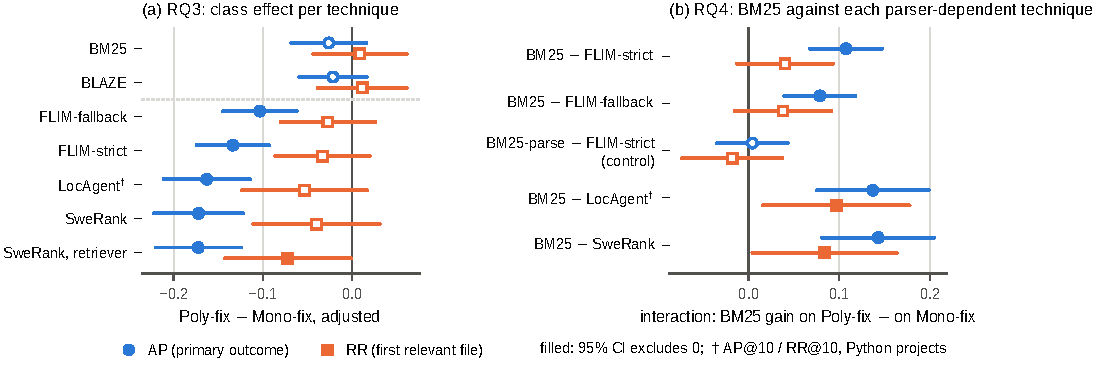
\includegraphics[width=\textwidth]{figures/fig_effects.pdf}
\caption{(a) RQ3: adjusted class effect (Poly-fix minus Mono-fix) per technique, on AP and on RR; techniques above the dashed line read every file. (b) RQ4: interaction of BM25 with each parser-dependent technique (BM25's gain on Poly-fix bugs minus its gain on Mono-fix bugs). Linear mixed models with $n_{\mathrm{gt}}$, $\log n_{\mathrm{cand}}$, report length, fold and a project random intercept; 95\% confidence intervals. All outcomes are in Tables~\ref{tab:rq3models} (Appendix~\ref{app:rq234}) and~\ref{tab:rq4}.}
\label{fig:effects}
\end{figure*}

\subsection{RQ3: Mono-fix vs Poly-fix performance}\label{sec:rq3}

The comparison pools the 1{,}399 primary-anchored test bugs of both folds (981
Mono-fix, 418 Poly-fix); LocAgent and SweRank use the 781 of the Python
projects (510 and 271). Figure~\ref{fig:effects}a gives the adjusted class
effects; per-project results and all outcomes are in
Appendix~\ref{app:rq234}.

\paragraph{The penalty depends on what the technique can read.} FLIM-strict
reaches a MAP of 0.370 on Mono-fix and 0.245 on Poly-fix bugs (adjusted class
effect $-0.134$, 95\% CI $[-0.174, -0.093]$) and ranks Poly-fix bugs lower in
five of the six projects. The two LLM-based techniques, which see Python files
only, have the largest penalties: LocAgent reaches an AP@10 of 0.456 and 0.253
($-0.163$ $[-0.211, -0.115]$), SweRank a MAP of 0.477 and 0.277 ($-0.172$
$[-0.222, -0.122]$). For BM25 and BLAZE, which index every file, the effect is
smaller and its interval includes 0 ($-0.026$ $[-0.068, 0.016]$ and $-0.021$
$[-0.059, 0.017]$). This is not evidence of no drop: equivalence within
$\pm0.05$ cannot be shown (TOST $p=0.13$ and $0.07$), so a drop of up to about
half of FLIM-strict's is compatible with the data. Restricting BM25 to
parseable files produces the same penalty as FLIM-strict ($-0.129$): the
penalty of the parseable view is a property of the candidate set, not of
FLIM's model, and text windows (FLIM-fallback) recover only a quarter of it
($-0.103$). The parser-dependent effects survive false-discovery control
($q<0.001$), a fractional-logit model, and a comparison of bugs with the same
number of ground-truth files (FLIM-strict $-0.102$, LocAgent $-0.113$,
SweRank $-0.109$; BM25 $-0.024$).

\paragraph{First-hit metrics weaken it.} BM25, FLIM and BLAZE have a
\emph{higher} raw MRR on Poly-fix than on Mono-fix bugs (FLIM-strict 0.513
against 0.466). After adjustment no class effect on RR excludes 0, and on
Top-10 only FLIM-strict's does ($-0.067$, half its effect on AP). A Poly-fix
bug almost always has a primary-language file, so its first relevant file is
found about as early as a Mono-fix bug's; what differs is the rest of the fix,
where complete-fix recall@10 falls by 0.178 for FLIM-strict and 0.190 for
SweRank, and not significantly for BM25 or BLAZE.

\begin{figure}[pos=t]
\centering
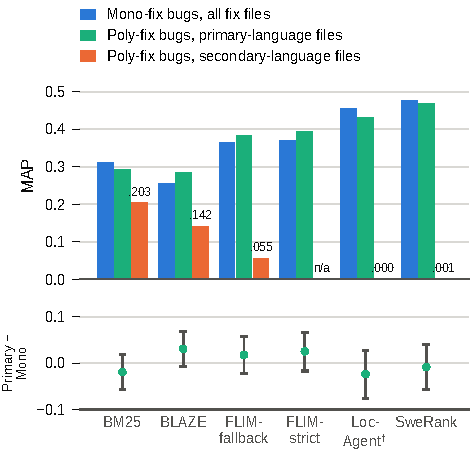
\includegraphics[width=\linewidth]{figures/fig_decomp.pdf}
\caption{Where the Poly-fix penalty comes from (both folds): MAP on the files of Mono-fix bugs, and on the primary-language and the secondary-language ground-truth files of Poly-fix bugs, each with the bug's other ground-truth files removed from the ranking. Lower panel: difference between the Poly-fix primary-language bar and the Mono-fix bar, with its 95\% bootstrap interval. FLIM-strict cannot rank secondary files. $^{\dagger}$Python projects, AP@10.}
\label{fig:decomp}
\end{figure}

\paragraph{The penalty comes from the secondary-language files.} On the
primary-language files of Poly-fix bugs no technique's MAP differs detectably
from its Mono-fix MAP (Figure~\ref{fig:decomp}, lower panel; e.g.\
FLIM-strict 0.395 against 0.370, SweRank 0.468 against 0.477), although the
intervals leave room for differences of 0.06--0.08. On the secondary files the
techniques separate, and this is the representation limit: BM25 reaches a MAP
of 0.203, BLAZE 0.142 and FLIM-fallback 0.055, while LocAgent and SweRank,
which cannot see them, reach 0.000 and 0.001. FLIM-fallback sees the same text
as BM25 but ranks these files almost four times lower: its encoder is
fine-tuned on the functions the fix changed, and most of its IR features use
parser output. BLAZE-all, trained on all fix files, has the same class effect
as BLAZE ($-0.031$), so its ranking of secondary files is not limited by not
having seen them in training.

\paragraph{Sub-types and conditions.} The FLIM-strict penalty is larger for
behaviour-bearing Poly-fix bugs ($-0.156$) than for test-asset-only ones
($-0.113$), and so is SweRank's ($-0.169$, $-0.147$); BM25 shows none for
either. Without test files in the ground truth (S1) the penalties shrink but
remain (FLIM-strict $-0.080$, SweRank $-0.094$). At the strict grain, where
the fix spans two programming languages, every technique is penalised (BM25
$-0.100$, FLIM-strict $-0.202$, SweRank $-0.212$). SweRank's reranker raises
both classes by the same amount (gains equivalent within $\pm0.03$,
$p=0.017$), so its language model does not change the penalty. In localstack,
where most Poly-fix fixes change a recorded test snapshot stored next to the
test that records it, Poly-fix bugs score higher for BM25 and BLAZE. Seed
variation (SD 0.012--0.030 MAP) is a fifth or less of the effects
(Appendix~\ref{app:runs}).

\begin{tcolorbox}[title=Answer to RQ3]
\poly bugs are localized worse than \mono bugs by every parser-dependent
technique: FLIM (adjusted MAP difference $-0.13$ strict, $-0.10$ with a text
fallback) and the two LLM-based techniques that see only Python files
(LocAgent $-0.16$ AP@10, SweRank $-0.17$ MAP). For the techniques that index
every file the drop is smaller and not significant (BM25 $-0.03$, BLAZE
$-0.02$), though not shown to be negligible. The difference lies mainly in the
secondary-language files, which the techniques that can read them rank
poorly. When a fix spans two programming languages, every technique is
penalised. MRR shows no adjusted class effect, and Top-10 about half of it.
\end{tcolorbox}

\subsection{RQ4: Classical retrieval against the parser-dependent techniques}\label{sec:rq4}

Differences here are BM25 minus the other technique, so a positive value
favours BM25 and a positive interaction means BM25 gains more on Poly-fix than
on Mono-fix bugs (Figure~\ref{fig:effects}b, Table~\ref{tab:rq4}).

% generated by Scripts/analysis/paper_tables.py -- do not edit
\begin{table*}[t]
\caption{RQ4: paired differences between techniques on the same bugs (both folds). $\bar d$ is the mean per-bug difference A $-$ B within a class; the interaction is the Poly-fix minus Mono-fix difference of $d$, adjusted as in Table~\ref{tab:rq3models}. The inversion pattern is $\bar d_{\mathrm{Mono}}<0\le\bar d_{\mathrm{Poly}}$: the parser-dependent technique is better on Mono-fix bugs and no better on Poly-fix bugs.}
\label{tab:rq4}
\footnotesize
\begin{adjustbox}{max width=\linewidth}\begin{tabular}{llrrrlc}
\toprule
Pair (A $-$ B) & Outcome & Bugs & $\bar d$ Mono & $\bar d$ Poly & Interaction [95\% CI] & Inversion \\
\midrule
BM25 $-$ FLIM-strict & AP & 1399 & $-$.059 & +.029 & +.107$^{*}$ [+.068, +.147] & yes \\
 & CFR@10 &  & $-$.084 & +.046 & +.150$^{*}$ [+.099, +.201] & yes \\
 & RR &  & $-$.077 & $-$.077 & +.040 [$-$.013, +.093] & no \\
 & Top-10 &  & $-$.099 & $-$.042 & +.096$^{*}$ [+.030, +.162] & no \\
\addlinespace
BM25 $-$ FLIM-fallback & AP & 1399 & $-$.054 & +.002 & +.079$^{*}$ [+.040, +.118] & yes \\
 & CFR@10 &  & $-$.074 & +.018 & +.111$^{*}$ [+.060, +.162] & yes \\
 & RR &  & $-$.073 & $-$.075 & +.038 [$-$.015, +.091] & no \\
 & Top-10 &  & $-$.087 & $-$.037 & +.088$^{*}$ [+.023, +.153] & no \\
\addlinespace
BM25-parseable $-$ FLIM-strict (control) & AP & 1399 & $-$.009 & $-$.026 & +.004 [$-$.035, +.043] & no \\
 & CFR@10 &  & $-$.041 & $-$.035 & +.017 [$-$.032, +.066] & no \\
 & RR &  & $-$.017 & $-$.067 & $-$.018 [$-$.073, +.037] & no \\
 & Top-10 &  & $-$.048 & $-$.061 & +.009 [$-$.054, +.072] & no \\
\addlinespace
BM25 $-$ LocAgent$^{a}$ & AP@10 & 781 & $-$.114 & +.036 & +.137$^{*}$ [+.075, +.199] & yes \\
 & CFR@10 &  & $-$.007 & +.143 & +.147$^{*}$ [+.074, +.219] & yes \\
 & RR@10 &  & $-$.246 & $-$.144 & +.097$^{*}$ [+.016, +.178] & no \\
 & Top-10 &  & $-$.126 & $-$.026 & +.080 [$-$.008, +.169] & no \\
\addlinespace
BM25 $-$ SweRank$^{b}$ & AP & 781 & $-$.113 & +.042 & +.143$^{*}$ [+.081, +.205] & yes \\
 & CFR@10 &  & $-$.018 & +.113 & +.151$^{*}$ [+.077, +.224] & yes \\
 & RR &  & $-$.264 & $-$.187 & +.084$^{*}$ [+.004, +.163] & no \\
 & Top-10 &  & $-$.149 & $-$.089 & +.050 [$-$.039, +.139] & no \\
\bottomrule
\end{tabular}\end{adjustbox}
\\[2pt]{\footnotesize $^{a}$Python projects; both techniques evaluated on their top ten files. $^{b}$Python projects; full rankings.}
\end{table*}


\paragraph{BM25 against FLIM.} On Mono-fix bugs FLIM-strict outperforms BM25
(mean per-bug AP difference $-0.059$); on Poly-fix bugs it loses that lead and
BM25 is slightly ahead ($+0.029$, 90\% interval $[0.008, 0.050]$; FDR-adjusted
$q=0.026$). The difference lies inside $\pm0.05$ (TOST $p=0.04$) but not
inside $\pm0.03$ ($p=0.46$). The interaction is $+0.107$ $[0.068, 0.147]$, and
complete-fix recall@10 shows the same ($+0.150$). On RR FLIM-strict leads by
0.077 in both classes, so the metric most often reported shows no reversal.
When BM25 is also restricted to parseable files, the interaction is
indistinguishable from 0 ($+0.004$ $[-0.035, 0.043]$): the loss of FLIM's lead
is caused by the ground-truth files it cannot reach, not by Poly-fix reports
being harder for its model. The pattern is carried by behaviour-bearing
Poly-fix bugs (BM25 ahead by 0.074; interaction $+0.138$); without test files
in the ground truth FLIM-strict stays ahead in both classes, but its lead
shrinks from 0.056 to 0.026 (interaction $+0.047$ $[0.005, 0.089]$).

\paragraph{BM25 against LocAgent and SweRank.} On the 781 Python test bugs
LocAgent outperforms BM25 on Mono-fix bugs (AP@10 0.456 against 0.342) and
loses that lead on Poly-fix bugs (0.253 against 0.289; not significant,
$q=0.25$); the interaction is $+0.137$ $[0.075, 0.199]$. LocAgent returns a
secondary-language file for almost no bug, so on Poly-fix bugs it finds the
Python part of the fix and nothing else. SweRank outperforms BM25 on Mono-fix
bugs by 0.113 MAP, more than any other technique, and loses that lead on
Poly-fix bugs (0.277 against 0.319; $q=0.18$); its interaction, $+0.143$
$[0.081, 0.205]$, is the largest in the study. Both lead on RR in both
classes. In ansible both lead BM25 in both classes, by less on Poly-fix bugs.

\paragraph{Sensitivity.} The BM25--FLIM-strict interaction keeps its sign and
excludes 0 under every condition except the filter-excluded bugs, whose
Poly-fix sample is small, and the control interaction includes 0 under every
condition. The LocAgent and SweRank interactions are not distinguishable from 0
without test files in the ground truth or at the strict grain
(Appendix~\ref{app:rq234}).

\begin{tcolorbox}[title=Answer to RQ4]
Largely yes, on the primary outcome. FLIM outperforms BM25 on \mono bugs and
loses that lead on \poly bugs, where BM25 is slightly ahead (interaction
$+0.11$ MAP); whether the two \emph{match} depends on the margin (within
$\pm0.05$, not shown within $\pm0.03$). The pattern is carried by
behaviour-bearing \poly bugs, is absent when BM25 is given only the files FLIM
can parse, and becomes a narrowing when tests are removed from the ground
truth. LocAgent ($+0.14$ AP@10) and SweRank ($+0.14$ MAP) show the same
interaction and lose their lead on \poly bugs without falling significantly
behind BM25. On RR all three lead BM25 on both classes.
\end{tcolorbox}

\subsection{RQ5: Reach or representation}\label{sec:variants}

RQ2--RQ4 leave open whether the parser-dependent techniques lose the
secondary files only because they cannot see them (reach) or would also rank
them poorly if they could (representation). The diagnostic variants give the
techniques those files (Table~\ref{tab:variants}). RQ5 is exploratory: it was
added after the results of RQ3 and RQ4 were known.

% generated by Scripts/analysis/paper_tables.py -- do not edit
\begin{table*}[pos=t]
\caption{RQ5, reach or representation: diagnostic variants of the parser-dependent techniques (ours, untuned; not proposed as techniques). A hybrid ranks the files the technique can represent by its own ranking and every other file by BM25, merged by reciprocal rank fusion ($k{=}60$); a co-change variant ranks the other files instead by how often they changed together with the technique's top five files before the report. ``All text files'' gives SweRank every candidate file: its own function documents plus 50-line chunks (at most 40 per file) of all other files; the indented rows add only the non-Python files, only the Python test files, or all files with at most 10 chunks each (retriever), and only the non-Python files (full SweRank). MAP of Mono-fix and Poly-fix bugs and of both together, MAP on the secondary-language files of Poly-fix bugs (other ground-truth files removed from the ranking), and the adjusted class effect as in Table~\ref{tab:rq3models} ($^{*}$: 95\% CI excludes 0).}
\label{tab:variants}
\footnotesize
\begin{adjustbox}{max width=\linewidth}\begin{tabular}{lrrrrrl}
\toprule
Technique & Bugs & MAP Mono & MAP Poly & MAP all & MAP sec. & Class effect [95\% CI] \\
\midrule
\multicolumn{7}{l}{\emph{All six projects (AP)}} \\
\quad BM25 & 1399 & .311 & .274 & .300 & .203 & $-$.026 [$-$.068, +.016] \\
\quad FLIM-strict & 1399 & .370 & .245 & .332 & n/a & $-$.134$^{*}$ [$-$.174, $-$.093] \\
\quad Hybrid: FLIM-strict + BM25 & 1399 & .349 & .296 & .333 & .140 & $-$.050$^{*}$ [$-$.091, $-$.009] \\
\quad Co-change: FLIM-strict + history & 1399 & .324 & .306 & .319 & .170 & $-$.025 [$-$.065, +.015] \\
\multicolumn{7}{l}{\emph{Python projects (AP@10)}} \\
\quad BM25 & 781 & .342 & .289 & .324 & .213 & $-$.026 [$-$.080, +.028] \\
\quad LocAgent & 781 & .456 & .253 & .386 & .000 & $-$.163$^{*}$ [$-$.211, $-$.115] \\
\quad Hybrid: LocAgent + BM25 & 781 & .488 & .349 & .440 & .123 & $-$.101$^{*}$ [$-$.153, $-$.048] \\
\quad Co-change: LocAgent + history & 781 & .449 & .314 & .402 & .101 & $-$.093$^{*}$ [$-$.147, $-$.040] \\
\multicolumn{7}{l}{\emph{Python projects (AP)}} \\
\quad BM25 & 781 & .364 & .319 & .349 & .226 & $-$.030 [$-$.082, +.023] \\
\quad SweRank retriever (Python functions) & 781 & .415 & .227 & .350 & .001 & $-$.172$^{*}$ [$-$.220, $-$.125] \\
\quad \quad + non-Python files only & 781 & .386 & .335 & .369 & .285 & $-$.023 [$-$.073, +.028] \\
\quad \quad + Python test files only & 781 & .526 & .289 & .444 & .001 & $-$.207$^{*}$ [$-$.263, $-$.151] \\
\quad SweRank retriever, all text files & 781 & .497 & .395 & .461 & .252 & $-$.063$^{*}$ [$-$.121, $-$.005] \\
\quad \quad at most 10 chunks per file & 781 & .482 & .372 & .444 & .216 & $-$.074$^{*}$ [$-$.130, $-$.018] \\
\quad SweRank (Python functions, as published) & 781 & .477 & .277 & .408 & .001 & $-$.172$^{*}$ [$-$.222, $-$.122] \\
\quad \quad + non-Python files only & 781 & .463 & .397 & .440 & .261 & $-$.020 [$-$.072, +.031] \\
\quad SweRank, all text files & 781 & .583 & .475 & .546 & .257 & $-$.044 [$-$.102, +.013] \\
\quad Hybrid: SweRank + BM25 & 781 & .509 & .380 & .465 & .128 & $-$.110$^{*}$ [$-$.164, $-$.056] \\
\quad Co-change: SweRank + history & 781 & .498 & .400 & .464 & .162 & $-$.082$^{*}$ [$-$.135, $-$.029] \\
\bottomrule
\end{tabular}\end{adjustbox}
\end{table*}


\paragraph{Given every file, SweRank ranks the secondary files at least as well
as BM25.} With all text files in its corpus, SweRank ranks the
secondary-language files of Poly-fix bugs at a MAP of 0.257, against 0.001 as
published and 0.226 for BM25 on the same bugs; it is not shown to be better
than BM25 but is non-inferior within 0.03 ($p=0.004$). For behaviour-bearing
files (66 bugs) the data cannot tell (Appendix~\ref{app:rq5}). Because SweRank
also ranks the Python files better, MAP over all bugs rises from 0.408 to
0.546, by 0.106 on Mono-fix and 0.198 on Poly-fix bugs (interaction $+0.126$
$[0.084, 0.168]$). The adjusted class effect falls by about three quarters,
from $-0.172$ to $-0.044$ $[-0.102, 0.013]$; a penalty of up to 0.10 remains
compatible with the data. SweRank on all files outperforms BM25 on both
classes, and its interaction with BM25 is indistinguishable from 0 ($+0.015$
$[-0.042, 0.072]$).

\paragraph{The non-Python files reduce the penalty; the Python test files do
not.} Adding only the non-Python files to the full technique gives an
interaction of $+0.153$ $[0.131, 0.176]$: Poly-fix MAP rises by 0.120 (0.277 to
0.397), and Mono-fix MAP falls by 0.015 because the added files compete with
the fixed Python files, so part of the narrower gap comes from the Mono-fix
side. The class effect falls to $-0.020$ $[-0.072, 0.031]$ (equivalence within
$\pm0.05$ not shown, $p=0.13$). Adding only the Python test files raises both
classes, Mono-fix more ($+0.111$ against $+0.062$, retriever), because test
files are in the ground truth of many Mono-fix fixes too. The reduction thus
comes from the secondary-language files, the reach explanation of RQ2.

\paragraph{Techniques that already see the files rank them below BM25.}
FLIM-fallback and BLAZE can read every file, yet rank the secondary files at a
MAP of 0.055 and 0.142 against 0.203 for BM25 (paired differences $0.148$
$[0.120, 0.178]$ and $0.062$ $[0.031, 0.094]$), for behaviour-bearing files and
test assets alike. For them representation is a limit in addition to reach.
We do not read the contrast with SweRank as one between newer and older
techniques: SweRank is a larger model trained on many repositories and applied
without project-specific training, whereas FLIM and BLAZE are fine-tuned per
project on a few hundred bugs whose fixed files are mostly source files, and
the comparison cannot separate these factors.

\paragraph{Filling in the missing files from BM25 or from history.} A hybrid
with BM25 raises every technique on Poly-fix bugs (FLIM-strict by 0.051,
LocAgent by 0.096 AP@10, SweRank by 0.103) and narrows the class effects to
$-0.050$, $-0.101$ and $-0.110$. Over all bugs it adds 0.054 to LocAgent and
0.057 to SweRank, but nothing to FLIM-strict ($+0.001$), for which it only
moves accuracy from Mono-fix to Poly-fix bugs. The co-change variant gives
similar Poly-fix gains and ranks the missing files better than the hybrid for
FLIM-strict and SweRank, but is not better over all bugs for any technique.
Neither recovers what SweRank achieves when it ranks those files itself
(Appendix~\ref{app:rq5}).

\begin{tcolorbox}[title=Answer to RQ5]
For SweRank the penalty is mainly one of reach. Given every text file, it
ranks the secondary files at least as well as BM25 (non-inferior within 0.03),
and its \poly penalty falls by about three quarters; the non-Python files
account for the reduction, while the Python test files raise both classes.
FLIM and BLAZE, which already see these files, rank them below BM25, so for
them representation is a limit as well. A hybrid with BM25 or with the change
history recovers part of the \poly loss for every parser-dependent technique,
and raises MAP over all bugs for LocAgent and SweRank, not for FLIM-strict.
\end{tcolorbox}

\subsection{No-primary and filter-excluded bugs}\label{sec:removed}

The 287 no-primary test bugs are the extreme case: no ground-truth file is in
the primary language, so FLIM and LocAgent can reach none. BM25 reaches a MAP
of 0.165 on them and BLAZE 0.091. Counting them changes the overall
comparison: over the primary-anchored and no-primary test bugs together,
FLIM-strict and BM25 are level (MAP 0.276 and 0.277, equivalent within
$\pm0.03$, $p<0.001$), whereas over the primary-anchored bugs alone
FLIM-strict leads (0.332 against 0.300). This also holds without
dolphinscheduler's front-end fixes, which a Java benchmark would usually
leave out. On the 432 filter-excluded test bugs every technique scores higher
than on the primary-anchored bugs and FLIM gains most, so BeetleBox's filter
did not remove the bugs on which classical retrieval is comparatively
strongest; the BM25--FLIM interaction has the sign of the main result but,
with 68 Poly-fix bugs, an interval that includes 0 (Appendix~\ref{app:removed}).

%% ===================================================================
%% 5 DISCUSSION
%% ===================================================================
\section{Discussion}\label{sec:discussion}

\paragraph{For the evaluation of bug localization.} A benchmark whose ground
truth contains only source files of the project language measures a
parser-dependent technique on the part of the task it can read. In our data
that part excludes about two-fifths of the files Poly-fix fixes change, and
Poly-fix bugs are 8--27\% of the primary-anchored bugs. On Mono-fix bugs FLIM
improves on BM25; on Poly-fix bugs it does not, and once the no-primary bugs
are counted it is level with BM25 overall. SweRank leads BM25 by 0.11 MAP on
Mono-fix bugs and loses that lead on Poly-fix bugs. A source-only ground truth
would report the first result for both. The metric matters as much: because
almost every Poly-fix fix also changes a primary-language file, MRR and Top-$k$
weaken every effect we report and show none of the reversals. We recommend
reporting AP or complete-fix recall when fixes contain several files, results
per fix class, and the share of the ground truth each technique can represent;
the class follows from the fix commit's file list, and reachability from the
technique's parser.

\paragraph{For technique design.} For SweRank, what the parser-dependent design
loses is mainly reach: given every text file it ranked configuration, data and
test assets at least as well as BM25 without any change to its models. The
choice that cost it the secondary files is in the corpus, not the model.
LocAgent's graph and keyword index make the same choice, which is why its
tools cannot return a YAML or JSON file however the model reasons. For FLIM
and BLAZE, which see these files but rank them below BM25, reach alone is not
enough. Whether SweRank's advantage here comes from its size, its pretraining
or the absence of per-project fine-tuning, a design study would have to vary
separately. Building the index from every text file rather than from parser
output recovered most of the loss for SweRank and raised its MAP over all bugs
by 0.138; where that is not possible, filling in the missing files from
lexical retrieval or the change history recovers part of it. Both are untuned
diagnostics, not proposed techniques.

\paragraph{For benchmark construction.} Indexing and scoring only source files
of the project language, as Bench4BL does \citep{lee2018bench4bl}, removes
the secondary files from the task, and with them the condition under which
parser-dependent techniques lose their advantage. Releasing the full file list
of each fix commit with a category per file, as we do, lets users choose the
ground truth and report the choice. Filters should be released with the data
they remove, as BeetleBox does: its filter of reports that name a fixed file,
usually seen as favouring lexical retrieval \citep{kochhar2014potential},
raised the Poly-fix share by 2.6 points and removed bugs that favour the
learned technique.

%% ===================================================================
%% 6 THREATS TO VALIDITY
%% ===================================================================
\section{Threats to Validity}\label{sec:threats}

\paragraph{Construct validity.} Language is attributed from file extensions.
The class and the ground truth come from the same fix files, but the fix
commit may contain unrelated changes (tangling; \citealt{herzig2013impact}).
Poly-fix fixes are larger and so more likely to be tangled, and a tangled
secondary file would both create the class and cause the penalty. Removing
merge commits (S4) leaves the results unchanged but does not address
squash-merged pull requests; \pending{manual tangling audit of a sample of
Poly-fix and Mono-fix fixes and the main models without the unrelated files}.
The prevalence depends on the boundary rules and is reported as a range.
Parseability is measured with one parser per language. The ground truth is
the change set rather than the fault location; the fault-oriented views (S1,
behaviour-bearing bugs) weaken several results. Assigning each project one
primary language is itself a monolingual assumption: dolphinscheduler's 520
front-end-only fixes become no-primary bugs.

\paragraph{Internal validity.} BLAZE is trained from a public checkpoint
because it was developed with BeetleBox. The chronological, purged split
prevents temporal leakage, and one evaluator scores every technique on the
same files. We did not reproduce any technique's published numbers on its own
benchmark, so an implementation problem cannot be ruled out that way, and
BLAZE is weaker than BM25 in our within-project setting, so its small class
effect could partly be a floor effect; the claim that reading every file
avoids the penalty rests mainly on BM25. Seed variance was measured on three
projects only. The pre-trained models may have seen these public repositories:
in a closed-book probe the LocAgent model named a correct file among ten for
at most 7.1\% of Mono-fix and 3.3\% of Poly-fix bugs, an asymmetry that could
slightly inflate the interaction; SweRank's training set is not released and
cannot be checked, but its models were fine-tuned on Python functions only, so
its ranking of non-Python files in RQ5 cannot come from memorised fine-tuning
targets (Appendix~\ref{app:runs}). AP is bounded and often 0 but modelled
linearly, and the random intercept rests on six projects (three for the
LLM-based techniques); a fractional-logit model gives the same estimates and
significance for every class effect and interaction.

\paragraph{External validity.} One dataset, two languages and six purposively
selected projects cannot represent Java and Python projects in general. Our
selection favoured projects whose fixes span several file types, and the
effect is visible within BeetleBox: in the seven eligible projects we did not
select, broad-grain prevalence is 18.5\% against 27.4\%
(Appendix~\ref{app:rq1}). Our prevalence figures are therefore upper values
for BeetleBox, and the localization results rest on the six projects.
Per-project Poly-fix test sets contain 38--121 bugs, so per-project results
are descriptive. LocAgent and SweRank run on three projects with their Small
or 7B models, not the largest variants, and in ansible both lead BM25 in both
classes, so only the interaction, not the reversal, holds in every project.
Other parser-dependent techniques may degrade differently, but the three we
ran span four years and three designs and show the same interaction. The
diagnostic variants are untuned, so their gains are lower bounds of what such
designs could reach. The 50-bug agreement check of the classification
\pending{human two-person round; Cohen's $\kappa$}.

%% ===================================================================
%% 7 CONCLUSION
%% ===================================================================
\section{Conclusion}\label{sec:conclusion}

Between 8\% and 27\% of the bug fixes in six Java and Python projects change
files of more than one language, depending on which files count; the extra
files are mostly configuration, data and test assets. A parser-dependent
localization technique cannot represent about two-fifths of the files those
fixes change and localizes those bugs worse, while for techniques that index
every file the drop is smaller and not significant. On these bugs the
parser-dependent techniques---FLIM, an agent and the most recent ranker in the
study---lose the lead they hold over classical retrieval on single-language
fixes, and the first-hit metrics the field reports most often hide it. For
SweRank the penalty is mainly a matter of reach: given every text file it
ranks the non-Python files at least as well as BM25 and its penalty falls by
about three quarters. Evaluations that keep only source files of the project
language therefore report the performance of parser-dependent techniques on
the part of the task they can read. We release the classification, the
per-file parse status, the score files and the analysis scripts so that other
techniques can be placed on the same footing.


%% ===================================================================
%% DECLARATIONS
%% ===================================================================
\section*{CRediT authorship contribution statement}
\pending{as in Objective 1.}

\section*{Declaration of competing interest}
The authors declare that they have no known competing financial interests or
personal relationships that could have appeared to influence the work reported
in this paper.

\section*{Declaration of generative AI and AI-assisted technologies in the writing process}
\pending{Statement as required by the venue.}

\section*{Data Availability}
The code---classifier, technique adapters, evaluator, statistics, and the
scripts that generate every table and figure---is in the GitHub repository
\url{https://github.com/eashaan-rao/polyglot-bug-localization}. The archived
replication package \pending{Zenodo DOI} contains that code and the data: the
frozen classification ruleset (0.2.0) and the per-bug and per-file
classification of all 4{,}995 bugs, the annotation protocol and agreement
material, the file universe and per-file parse status of every evaluated
snapshot, the chronological splits, the score file of every technique, fold
and seed with its run manifest, the trained FLIM, BLAZE and BLAZE-all models,
the LocAgent outputs and trajectories, the SweRank retrieval and reranking
outputs with every LLM response, and the outputs of the diagnostic variants.

\bibliographystyle{cas-model2-names}
\bibliography{refs}

\clearpage
%% ===================================================================
%% APPENDICES (supplementary material)
%% ===================================================================
\appendix
\section{Related work: positioning}\label{app:related}

\begin{table*}[t]
\caption{Positioning: what each line of work provides and what this study adds.}
\label{tab:positioning}
\small
\begin{adjustbox}{max width=\linewidth}\begin{tabular}{p{3.3cm}p{6.2cm}p{6.6cm}}
\toprule
Line of work & Strength we use & Gap this study addresses \\
\midrule
Fix characterisation & Method for classifying fixes; multi-hunk taxonomy & Classifies by size and distance, not by file type \\
Cross-language BL (BLAZE, BeetleBox) & Multi-language ground truth; language-agnostic technique & Unit is a single-language fix within a project \\
Language-interaction bugs (xLoc) & Bugs at language boundaries & Bugs \emph{caused} by a boundary, not fixes that \emph{cross} one \\
Dataset quality & Ground truth affects measured performance & Concerns files wrongly included, not files fixes contain \\
Polyglot SE / RTS & Monolingual tools can be unsafe on polyglot code & Different task (testing, not localization) \\
LLM-based localization (agents, rankers) & Current techniques; graph-based tools; retrieve-and-rerank & Evaluated on source-only targets (SWE-bench, LocBench) \\
\bottomrule
\end{tabular}\end{adjustbox}
\end{table*}

\section{Study-design details}\label{app:design}

\paragraph{Classification protocol.} A fifth criterion (C5) decides only which
languages receive their own row in the statistics: at least 15 Poly-fix bugs
across at least two projects.
The written protocol was checked on a stratified sample of 50 bugs before any
technique was run: annotators classify every fix file (counted or excluded,
language, test scope) and every bug (label, keep, secondary languages,
sub-type) from the protocol alone, without access to the classifier; the
two-person agreement is reported in Section~\ref{sec:classification}. A
preliminary round with two independent automated annotators following the
same protocol agreed with each other and with the ruleset on every bug-level
field; it led to publishing the exact path patterns in the protocol. Three
rule readings it questioned were kept frozen rather than amended; amending
them would change the Poly-fix label of at most 1.4\% of Poly-fix bugs. Test scope is decided from the path, so test-harness code in a \texttt{test} package under \texttt{src/main/} counts as test (96 primary-language ground-truth files); this affects only S1 and the sub-type.

\paragraph{Bugs outside the primary-anchored set.} Of the 4{,}995 bugs of the
six projects, 1{,}401 are not primary-anchored: 417 change no counted file (documentation or changelog only), and 984---21.5\% of
the 4{,}578 bugs with counted fix files---change counted files but none in the
primary language: 520 single-language fixes in another language (mostly the
TypeScript and Vue front-end of dolphinscheduler), 374 fixes of configuration,
schema or build files only, and 90 multi-language fixes without the primary
language. These no-primary fixes cannot enter the Mono-fix/Poly-fix
comparison, but they are the case in which a parser-dependent technique can
reach no fixed file at all, so we analyse them as a separate group
(Section~\ref{sec:removed}). The 1{,}226 filter-excluded reports are distributed as elasticsearch 363,
airflow 383, ansible 295, dolphinscheduler 83, localstack 63 and liquibase 39.

\paragraph{Why Java and Python.} The restriction is by design, not for lack of data: BeetleBox has more C++ and JavaScript bugs (5{,}268 and 3{,}783) than Java or Python bugs (3{,}707 and 3{,}759). The pair also covers a statically and a dynamically typed ecosystem.

\paragraph{Departures from the original implementations.} Table~\ref{tab:deviations} lists every departure of our runs from the authors' code. FLIM has 19 IR features in the original and 18 in our runs.

% moved from main.tex to the supplementary material (2026-11-09)
\begin{table*}[t]
\caption{Departures from the original implementations.}
\label{tab:deviations}
\small
\begin{adjustbox}{max width=\linewidth}\begin{tabular}{p{1.8cm}p{14.3cm}}
\toprule
Technique & Departure and reason \\
\midrule
BLAZE & Hard examples are weighted inside the batch by the loss; the paper's GPT-mined hard-example set is BeetleBox-specific. Comments are not stripped before chunking. The learning rate is selected by validation MAP from $\{2{\times}10^{-7}, 2{\times}10^{-6}, 2{\times}10^{-5}\}$ (the paper's value and two larger ones), because the paper's value was set for $\sim$11{,}000 training bugs and our projects have 100--600. Selected in fold~1: $2{\times}10^{-7}$ for liquibase and localstack, $2{\times}10^{-6}$ for dolphinscheduler, $2{\times}10^{-5}$ for elasticsearch, ansible and airflow; all selected values in the learning-rate table of the replication package. \\
FLIM & Positive pairs are the functions the fix changed (diff overlap), not every function of the fixed file. Its TF-IDF features split identifiers at camel-case boundaries without keeping the whole identifier. The CodeSearchNet pairs of the paper's MIX set are not added. IR feature f2 (API-enriched similarity) needs JDK documentation and has no Python counterpart, so it is dropped. Other positives of the same report are masked out of the in-batch loss. The learning rate is selected by validation MAP between the two published values ($2{\times}10^{-5}$ in the released code, $5{\times}10^{-5}$ in the paper). Selected in fold~1: $2{\times}10^{-5}$ for elasticsearch and airflow, $5{\times}10^{-5}$ for the other four projects; the learning-rate table of the replication package. \\
LocAgent & No change to prompts, tools or search logic. One bug in its driver is fixed: a tool output is passed to \texttt{eval()}, which fell back to the raw text only on a syntax error, so outputs beginning with a path such as \texttt{lib/ansible/\ldots} raised a name error, killed the worker and left the run waiting forever; the fix extends the existing fallback to every error, so every output that did not crash is handled exactly as before. An adapter exports our test bugs as LocAgent instances (pre-fix commit, report text; the patch field is left empty) and builds LocAgent's graph and BM25 indexes from our local clones with LocAgent's own builders, materialising the full commit tree (not \texttt{git archive}, which drops paths marked \texttt{export-ignore}), so LocAgent sees the same pre-fix snapshot as the other techniques. We use the paper's fine-tuned 7B model rather than its 32B model: the 32B bf16 weights (65.5\,GB) exceed our 48\,GB GPU, and loading them with on-the-fly FP8 quantization ran out of memory. The paper reports both; its ablations use the 7B model (file-level Acc@5 on SWE-bench Lite 88.3 for 7B, 92.7 for 32B). \texttt{litellm} 1.52.1, pinned by LocAgent, is no longer on PyPI; 1.53.1 is used. \\
SweRank & No change to the corpus builder, retriever, prompts, reranking loop or permutation parsing; reranking uses the authors' sequential path, one bug at a time. An adapter feeds the same bugs, pre-fix snapshots and report text as for LocAgent, and maps the reranked functions to files by first appearance; files beyond the top 100 functions keep the retriever's order. SweRank's structure builder files a snapshot's top-level files under the repository name, which collides with a package directory of the same name (\texttt{localstack/}, \texttt{airflow/}); file paths are resolved against the snapshot. A function text already embedded for an earlier bug of the same project is not embedded again. vLLM's memory share is lowered from 0.9 to 0.55 for our shared GPU. We use the Small models (7B reranker), a configuration documented in the released code, rather than the Large ones: the 32B reranker exceeds our GPU, as for LocAgent. A faster variant that sent the reranking prompts of many bugs to the GPU together did not reproduce the sequential order (0 of 6 bugs) and was not used. \texttt{pyarrow}, which the authors do not pin, is set to 20.0.0. \\
\bottomrule
\end{tabular}\end{adjustbox}
\end{table*}


\paragraph{Why these five.} FLIM is parser-dependent by architecture: it
cannot form its semantic features without the function list, and 13 of its
18 IR features use parser output. Of the other parser-based candidates,
BL-GAN \citep{zhu2022bl} represents an unparseable file by its path only and
is recorded in the feasibility analysis, but not run; TRANP-CNN
\citep{huo2019deep} treats text lines as statements without parsing and is
therefore language-agnostic in our sense. BL-GAN is not run end to end: its
behaviour on secondary files is fixed by its architecture (path only), so
running it would add a second technique with the same reach as FLIM-strict
rather than a different kind of technique, at the cost of a GAN training per project
and fold. Among the LLM-based techniques, LocAgent represents agents and
SweRank, published four years after FLIM and reported by its authors to
outperform agent-based localizers, represents learned rankers; it lets us ask
whether the newest parser-dependent technique behaves like the oldest.
Agentless \citep{xia2024agentless} is not run: it reads only Python files,
as LocAgent does, so it would not add a different reach, and its published
configuration uses GPT-4o, which cannot be run locally.

\paragraph{LocAgent, SweRank and Java.} Both LLM-based techniques read
Python only. LocAgent's graph builder uses Python's \texttt{ast}, and its BM25
index keeps only \texttt{.py} files outside test directories; all four of its
tools operate on these two indexes, so Python test files are reachable through
the graph but not through keyword search, and no non-Python file is reachable
at all. SweRank's corpus builder keeps the functions of \texttt{.py} files
whose path does not contain ``test''. Both techniques' models were trained on
Python data only, and SweRank's authors describe existing ranking approaches,
theirs included, as Python-centric; their multilingual SweRank+
\citep{reddy2025sweranplus} is not released (checked November 2026). Neither
can index the Java projects, which we report as a feasibility result, and we
run both on the Python projects only. Porting their parsers to Java would make
a new technique whose result could not be separated from the Python-only
training.

\paragraph{Test sets.} Fold~1 has 719 primary-anchored test bugs (483 Mono-fix, 213 Poly-fix and
23 that are multi-language only outside the broad grain); fold~2 has 718 (505,
206, 7). A bug whose fixed files were all added by the fix has nothing to rank
and is left out of the rank metrics, which leaves 1{,}399 Mono-fix and Poly-fix
test bugs over the two folds (981 and 418).

\paragraph{File universe.} For each test bug, every technique scores every
file of the pre-fix snapshot that is text (at most 1\,MB and no NUL byte in
its first 8\,KB). The \emph{primary universe} R keeps the files that the
classification ruleset counts; the \emph{text universe} T keeps all text files
and is used for sensitivity. There is no retrieval stage that pre-selects
candidates. The median R is 1{,}890 (localstack) to 21{,}658 (elasticsearch)
files per snapshot.

\paragraph{Change set rather than fault location.} The ground truth is the
change set of the fix, not only the location of the fault. We use it for three
reasons. A developer who acts on a localization result has to change every
file of the fix, and a file that is missing from the ranking is a file the
developer must find unaided. The standard benchmarks also derive their ground
truth from the files a fix changed \citep{lee2018bench4bl,jimenez2023swe}; they
differ from ours mainly in keeping only source files. And the class must be
defined on the same files as the target, or a bug could be Poly-fix by files
that are never scored. The change set includes files a fault-oriented reading
would exclude: recorded test snapshots, expected outputs and test
specifications that change because the behaviour changed. Two techniques,
LocAgent and SweRank, exclude test files by design. We therefore give equal
weight to two fault-oriented views of every result: the ground truth without
test files (sensitivity S1) and the behaviour-bearing Poly-fix bugs, whose
extra files are read by the software.

\paragraph{Metrics.} Per bug we compute the rank of each reachable
ground-truth file, Top-$k$ (whether a ground-truth file is ranked in the first
$k$, $k \in \{1,5,10\}$), the reciprocal rank of the first ground-truth file
(RR; its mean over bugs is MRR), average precision (AP; its mean is MAP; the
precision at each hit, summed and divided by the number of reachable
ground-truth files) and
complete-fix recall@10 (CFR@10: the share of a bug's reachable ground-truth
files in the first 10). Ties are resolved by expected rank under random tie-breaking.
For each bug we also compute the RR and Top-10 that random ranking would reach
given the number of candidates and ground-truth files.

\emph{Primary outcome.} AP, and its mean MAP, is the primary outcome;
complete-fix recall@10, RR and Top-$k$ are secondary. We fixed this before
any full run: every primary-anchored Poly-fix bug has a fix file in the primary language,
so a metric that rewards only the first ground-truth file (RR, Top-$k$) cannot
show whether a technique reaches the rest of the fix, whereas AP counts every
reachable ground-truth file. In the LocAgent trial, for example, a Poly-fix
bug had RR 1.0 and AP 0.25: the Python file was ranked first, and the YAML and
INI files of the fix were never returned. LocAgent returns a ranked list of
at most ten files, so comparisons that include it use AP@10 (ranks beyond 10
count as misses; still divided by the number of reachable ground-truth files,
so a bug with more than ten cannot reach 1) for every technique, with complete-fix recall@10, Top-$k$
and RR@10 secondary. LocAgent is run on the 395 fold-1 and 395 fold-2 test bugs of
the three Python projects, plus the filter-excluded bugs in those test windows (121
and 136). SweRank is run on exactly the same bugs. Unlike LocAgent it ranks
every non-test Python file that contains a function, so it is evaluated on AP
like BM25 and FLIM; the files it cannot see are left unscored and therefore
share the last ranks. Counting them as misses instead, as the parseable view
does for FLIM-strict, gives the same class effect ($-0.172$ in both views). Its retrieval stage alone, before the LLM reranks, is
evaluated as a second ranking from the same run (``SweRank, retriever only'').

\paragraph{Ablation and repeated runs.} To test whether a language-agnostic
technique's ranking of secondary files is limited by its training data, we
train BLAZE once more on chunks of \emph{all} fix files rather than only
project-language files (BLAZE-all; fold~1, seed 13, the learning rate selected
for BLAZE). LocAgent samples at temperature 1.0; we repeat it twice on a fixed
random subset of 100 fold-1 bugs to report run-to-run variation. SweRank
trains nothing and decodes greedily, so it is run once; because greedy
decoding on a GPU is not guaranteed to be bit-identical between runs, we re-run
it on a random subset of fold-1 bugs (20, plus one bug that differed in an
earlier check) to measure the variation.

\paragraph{Diagnostic variants: implementation.} Two kinds of variant
ask what the parser-dependent techniques would do with the files they cannot
represent. A \emph{hybrid} ranks the files a technique can represent by the
technique's own ranking and every other file by BM25, and merges the two
lists by reciprocal rank fusion with the standard constant $k{=}60$
\citep{cormack2009rrf}: a file at rank $r$ in its list scores $1/(60+r)$. We
build hybrids of FLIM-strict, LocAgent and SweRank from the stored score files.
A \emph{co-change} variant replaces BM25 by the project's history
\citep{zimmermann2004mining}: using only commits made before the report
(merges, the fix commit and commits that change more than 30 files excluded),
it scores every file the technique does not rank by how often it changed
together with the technique's top five files, $\sum_{a} c(a,b)/(n(a)\,r_a)$,
where $n(a)$ counts the commits that changed file $a$, $c(a,b)$ those that
changed both, and $r_a$ is $a$'s rank; the two lists are merged as for the
hybrid.
\emph{SweRank on all text files} keeps SweRank's own function documents and
adds every other candidate file of the snapshot---non-Python files, Python
test files and Python files without a function---as chunks of 50 lines in
SweRank's document format (path, then text), at most 40 chunks per file. We
run its retriever on this corpus and then its reranker on the top 100
documents, with the settings of the main run; a file's position is that of its
best document. To see which of the added files cause a change, we also run
the retriever on three partial corpora: SweRank's documents plus only the
non-Python files, plus only the Python test files, and plus all files with at
most 10 chunks each. On the first of these, the decisive one, we also run the
full technique, retriever and reranker, with the settings of the main run. None of the variants is tuned: the constant, the chunk
length and the caps were fixed before each run. The variants, and RQ5 itself,
were added after the results of RQ3 and RQ4 were known, so RQ5 is
exploratory; the partial corpora were added later still.
Each is compared with the
original technique and with BM25 on the same bugs, by its MAP over all bugs
and per class, by the paired tests and interaction models of RQ4, and by the
MAP of the secondary files with the other ground-truth files removed, split
into behaviour-bearing and test-asset files (Section~\ref{sec:definitions}).

\paragraph{Training budget and hyper-parameters.} Every hyper-parameter comes
from the authors' released code except the learning rate. The neural
techniques are trained up to their papers' epoch counts (BLAZE 15, FLIM 10),
with the epoch selected on the validation split by each technique's own
criterion (BLAZE: validation loss; FLIM: validation MRR) and an early-stopping
patience of 3 epochs. The learning rate is chosen for both techniques by one
rule: validation MAP, the primary outcome, over a small grid around the
published values ($\{2{\times}10^{-7}, 2{\times}10^{-6}, 2{\times}10^{-5}\}$
for BLAZE, whose $2{\times}10^{-7}$ was set for about 11{,}000 bugs pooled
across projects; $\{2{\times}10^{-5}, 5{\times}10^{-5}\}$ for FLIM, the
values of its code and paper). We do not select on the training loss, which
measures how a report separates its own chunks from about twenty in-batch
chunks rather than how a file ranks among thousands; in our pilot the two
criteria disagreed. The choice is made once per project and fold with the
first seed; the test set is never used. BLAZE selected the published rate in
five of twelve project--folds, the middle rate in two and the largest in five,
where the validation loss was lowest after one to four epochs, so a larger
rate would only over-fit sooner (Table~\ref{tab:lr}, with epochs and GPU cost).

Each neural technique is run with seed 13 on every project and fold, and with
seeds 42 and 2027 on fold~1 of localstack, dolphinscheduler and liquibase.
Bootstrap intervals and paired tests account for which bugs are in the test
set, not for the randomness of training, which repeated runs measure
\citep{arcuri2011practical}. Where several seeds exist, per-bug metrics are
averaged over them. BM25 is deterministic and run once.

% generated by Scripts/analysis/paper_tables.py -- do not edit
\begin{table*}[t]
\caption{Learning rate selected on validation MAP (seed 13) and, in parentheses, the selected epoch / epochs run before early stopping (BLAZE at most 15, FLIM at most 10).}
\label{tab:lr}
\footnotesize
\begin{adjustbox}{max width=\linewidth}\begin{tabular}{lllll}
\toprule
 & \multicolumn{2}{c}{BLAZE} & \multicolumn{2}{c}{FLIM} \\
\cmidrule(lr){2-3}\cmidrule(lr){4-5}
Project & fold 1 & fold 2 & fold 1 & fold 2 \\
\midrule
elasticsearch (J) & $2{\times}10^{-5}$ (1/4) & $2{\times}10^{-5}$ (4/7) & $2{\times}10^{-5}$ (2/5) & $2{\times}10^{-5}$ (6/9) \\
liquibase (J) & $2{\times}10^{-7}$ (15/15) & $2{\times}10^{-6}$ (8/11) & $5{\times}10^{-5}$ (6/9) & $2{\times}10^{-5}$ (3/6) \\
dolphinscheduler (J) & $2{\times}10^{-6}$ (12/15) & $2{\times}10^{-7}$ (11/14) & $5{\times}10^{-5}$ (2/5) & $2{\times}10^{-5}$ (9/10) \\
ansible (P) & $2{\times}10^{-5}$ (1/4) & $2{\times}10^{-7}$ (12/15) & $5{\times}10^{-5}$ (3/6) & $5{\times}10^{-5}$ (5/8) \\
airflow (P) & $2{\times}10^{-5}$ (1/4) & $2{\times}10^{-5}$ (1/4) & $2{\times}10^{-5}$ (3/6) & $2{\times}10^{-5}$ (6/9) \\
localstack (P) & $2{\times}10^{-7}$ (14/15) & $2{\times}10^{-7}$ (15/15) & $5{\times}10^{-5}$ (2/5) & $2{\times}10^{-5}$ (7/10) \\
\bottomrule
\end{tabular}\end{adjustbox}
\\[2pt]{\footnotesize Training and scoring cost on one NVIDIA L40 (all seeds): BLAZE: 18 runs, 74 GPU-hours; BLAZE-all: 6 runs, 13 GPU-hours; FLIM: 18 runs, 14 GPU-hours.}
\end{table*}


\paragraph{Statistical details.} $n_{\mathrm{gt}}$ is included because Poly-fix bugs have more ground-truth
files and Top-$k$ is easier with more targets. If the random-intercept model
cannot be fitted, we fall back to project fixed effects with HC3 standard
errors; with six projects, cluster-robust errors are not used (the fallback was
needed for 49 of 832 class-effect models and 97 of 380 interaction models,
never for a main AP analysis except the SweRank reranker comparison). A logistic
model on Top-10 with project fixed effects is the robustness check. Per-bug
metrics of the seeded techniques are averaged over seeds, and the two folds
are pooled with fold as a fixed effect. Because
$n_{\mathrm{gt}}$ differs strongly between the classes (4.3 against 2.4
reachable files on average), we also compare the classes within strata of
equal $n_{\mathrm{gt}}$ (1, 2, 3, 4, 5 or more), weighting each stratum by its
size, with a bootstrap interval. The false-discovery rate is controlled separately over all class-effect tests (832) and all interaction tests (380). LocAgent
is compared with BM25 on the Python projects with the same paired tests on
AP@10 (secondary: complete-fix recall@10, Top-10, RR@10), and SweRank on the
same bugs on AP (secondary: complete-fix recall@10, RR, Top-10). Comparing
SweRank with its own retriever separates what the LLM reranker contributes
from what the candidate set allows. Because
AP is bounded and has a mass at 0, we refitted the class-effect and
interaction models as fractional-logit regressions with project fixed
effects. The average marginal effects agree with the linear estimates (BM25
$-0.026$, BLAZE $-0.016$, FLIM-strict $-0.132$, LocAgent $-0.158$, SweRank
$-0.172$, SweRank on all files $-0.045$), each is significant exactly where the
linear one is, and every interaction keeps its sign and significance (the
parseable-view control: $p=0.95$). The statistics have further known limits: bootstrap intervals resample bugs and ignore correlation within a project over time, and bugs with several seeds enter the models as seed averages next to single-seed bugs.

\section{RQ1 details}\label{app:rq1}

Over all 4{,}995 bugs, including those whose fix changes no file in the primary language, the broad-grain share is 19.7\%. Every counted secondary file in the Poly-fix bugs is also in the dataset's ground truth (Table~\ref{tab:secondary}). The behaviour-bearing secondary files are mostly YAML (147
bugs), XML (88), JSON (51), TypeScript (47), JavaScript (41), INI (30), Shell
(25) and Gradle (21). By project, test-asset-only bugs make up 91.9\% of the Poly-fix bugs of ansible, 85.9\% of liquibase, 83.2\% of localstack and 70.3\% of elasticsearch, but 0.6\% of airflow and of dolphinscheduler.

Table~\ref{tab:sensitivity} reports how the broad-grain prevalence changes
when one boundary rule is changed at a time. Excluding test files reduces it
to 11.0\% and counting changelog fragments raises it to 41.3\%; counting
documentation or deletions changes it by at most 0.1 percentage points.
Restricting to programming languages gives the strict grain, 8.2\%.

Among the 1{,}226 bugs BeetleBox removed because their report names a fixed
file, 1{,}055 would be kept, and 15.9\% of those are Poly-fix at the
broad grain, against 27.4\% of the primary-anchored bugs; the share is lower in five of
the six projects (liquibase: 50.0\% against 49.7\%). Counting the filter-excluded bugs
as well gives 24.8\% (1{,}153 of 4{,}649). The dataset's filter therefore
raised the Poly-fix share of the primary-anchored set by 2.6 percentage points.

% moved from main.tex to the supplementary material (2026-11-09)
\begin{table}[t]
\caption{Secondary languages in Poly-fix bugs (primary-anchored bugs containing at least one such file).}
\label{tab:secondary}
\small
\begin{adjustbox}{max width=\linewidth}\begin{tabular}{lrr}
\toprule
Secondary language & Poly-fix bugs & Projects \\
\midrule
YAML & 497 & 6 \\
JSON & 163 & 6 \\
XML & 117 & 4 \\
Shell & 101 & 5 \\
Groovy & 72 & 2 \\
TypeScript & 47 & 2 \\
JavaScript & 43 & 3 \\
Gradle & 33 & 1 \\
SQL & 19 & 2 \\
17 further languages & 1--19 each & 1--3 \\
\bottomrule
\end{tabular}\end{adjustbox}
\end{table}

% moved from main.tex to the supplementary material (2026-11-09)
\begin{table}[t]
\caption{Sensitivity of Poly-fix prevalence (broad grain, share of primary-anchored bugs) to the boundary rules, one rule changed at a time.}
\label{tab:sensitivity}
\small
\begin{adjustbox}{max width=\linewidth}\begin{tabular}{lrr}
\toprule
Rule change & Poly-fix & \% \\
\midrule
None (default rules) & 985 & 27.4 \\
Only programming languages count & 294 & 8.2 \\
Exclude test files$^{a}$ & 365 & 11.0 \\
Count changelog fragments & 1{,}484 & 41.3 \\
Count documentation & 985 & 27.4 \\
Count deletions$^{b}$ & 989 & 27.5 \\
\bottomrule
\end{tabular}\end{adjustbox}
\\[2pt]{\footnotesize $^{a}$3{,}324 primary-anchored bugs under this rule. $^{b}$3{,}595 primary-anchored bugs. Merging data-configuration languages into one pseudo-language is a label-level check only (label-level prevalence unchanged at 28.7\%); it is not defined for the grains.}
\end{table}


\paragraph{Beyond the six projects.} To see how far the selection shapes these
figures, we classified the bugs of all 13 Java and Python projects of BeetleBox
with at least 100 reports in the same way (Table~\ref{tab:rq1all}). Re-running
the procedure on the six study projects reproduces the main classification for
all 4{,}995 bugs. The selection effect is the difference between the study
projects and the seven others, and it is substantial. Of the primary-anchored
bugs, 27.4\% are Poly-fix at the broad grain in the study projects against
18.5\% in the others (per-project medians 29.0\% and 17.5\%), and 21.0\%
against 8.5\% at the data-format grain. Only the strict grain is higher in
the others (10.6\% against 8.2\%), and this comes from two projects. The others
also differ in a second respect: only 35.7\% of their bugs with a counted
fix file are primary-anchored, against 78.5\% in the study projects. Counted
over all bugs with a counted fix file, broad-grain Poly-fix bugs are 21.5\% of
the study projects' bugs and 6.6\% of the others'.

Two of the seven are cases where a single primary language does not describe
the project. In ccxt only 40 of 674 bugs with counted files touch Python, and
in posthog 101 of 382; most of their fixes are in other languages. Their high
shares at the broad and strict grains (70.0\% and 36.6\% broad) describe these
small subsets, not the projects. Without them, the five remaining projects have
a broad-grain share of 12.8\% and a strict share of 4.1\% of 680
primary-anchored bugs. The proxy predicts prevalence only loosely (dubbo:
proxy 7.4\%, prevalence 7.5\%; openrefine, 29.4\% and 22.8\%).
Pooling all 13 projects gives 25.8\%, but 81\% of that pool are the study
projects' bugs, so it is not an independent estimate. Our prevalence figures
therefore describe projects selected to contain both classes and are upper
values for BeetleBox as a whole.

\begin{table}[t]
\caption{Poly-fix prevalence over all 13 Java and Python projects of BeetleBox with at least 100 bug reports (ruleset 0.2.0), the six study projects and the seven others.}
\label{tab:rq1all}
\small
\setlength{\tabcolsep}{3pt}
\begin{adjustbox}{max width=\linewidth}\begin{tabular}{lrrrrrrrr}
\toprule
 & & & & & \multicolumn{3}{c}{\% of anchored} & \% of cnt. \\
\cmidrule(lr){6-8}\cmidrule(lr){9-9}
Project & Bugs & Anch. & Anch.\,\% & Proxy & broad & data & strict & broad \\
\midrule
\multicolumn{9}{l}{\emph{Study projects}} \\
dolphinscheduler (J) & 1{,}363 & 698 & 53.6 & 29.4 & 23.6 & 14.6 & 10.7 & 12.7 \\
elasticsearch (J) & 970 & 721 & 84.8 & 49.4 & 17.8 & 15.1 & 0.3 & 15.1 \\
liquibase (J) & 241 & 199 & 84.7 & 42.7 & 49.7 & 20.1 & 35.7 & 42.1 \\
airflow (P) & 1{,}181 & 917 & 85.2 & 32.9 & 18.8 & 14.2 & 5.5 & 16.0 \\
ansible (P) & 768 & 626 & 94.7 & 66.0 & 43.5 & 39.1 & 13.4 & 41.1 \\
localstack (P) & 472 & 433 & 95.6 & 37.1 & 34.4 & 29.6 & 2.8 & 32.9 \\
\quad pooled & 4{,}995 & 3{,}594 & 78.5 & 41.1 & 27.4 & 21.0 & 8.2 & 21.5 \\
\midrule
\multicolumn{9}{l}{\emph{Other eligible projects}} \\
dubbo (J) & 379 & 253 & 67.8 & 7.4 & 7.5 & 5.5 & 0.0 & 5.1 \\
openrefine (J) & 620 & 189 & 34.9 & 29.4 & 22.8 & 16.9 & 13.8 & 7.9 \\
selenium (J) & 134 & 46 & 46.0 & 11.9 & 2.2 & 0.0 & 2.2 & 1.0 \\
ccxt (P) & 690 & 40 & 5.9 & 11.8 & 70.0 & 10.0 & 67.5 & 4.2 \\
langchain (P) & 130 & 112 & 97.4 & 26.2 & 8.9 & 2.7 & 0.0 & 8.7 \\
odoo (P) & 115 & 80 & 70.8 & 12.2 & 17.5 & 16.2 & 1.2 & 12.4 \\
posthog (P) & 403 & 101 & 26.4 & 48.6 & 36.6 & 4.0 & 31.7 & 9.7 \\
\quad pooled & 2{,}471 & 821 & 35.7 & 22.3 & 18.5 & 8.5 & 10.6 & 6.6 \\
\midrule
All 13 & 7{,}466 & 4{,}415 & 64.2 & 34.9 & 25.8 & 18.7 & 8.6 & 16.5 \\
\bottomrule
\end{tabular}\end{adjustbox}
\\[2pt]{\footnotesize Anch.: primary-anchored bugs; Anch.\,\%: their share of the bugs with a counted fix file. Proxy: share of fixes whose changed files have more than one extension (pooled: weighted by bugs). Prevalence in \% of primary-anchored bugs (``data'': data-format grain) and, in the last column, broad-grain Poly-fix bugs in \% of all bugs with a counted fix file. In ccxt and posthog fewer than a third of the bugs touch the assigned primary language, so their prevalence describes a small subset. The study projects re-classified by the same script agree with the main classification for all 4{,}995 bugs.}
\end{table}


\section{RQ2--RQ4 details}\label{app:rq234}

\paragraph{Reachability.} Table~\ref{tab:reach} gives the reachability of the ground-truth files before any technique is run. Of the reachable
ground-truth files of Poly-fix bugs, 62.8\% are parseable; for Mono-fix bugs
the share is 99.9\%. Because every primary-anchored bug has a primary-language fix file,
98.1\% of Poly-fix bugs still have at least one parseable ground-truth file,
but only 10.8\% have \emph{only} parseable ones. A parser-dependent technique
can therefore reach a Poly-fix bug, but on average not about 37\% of the
files its fix changes (40.8\% over all Poly-fix bugs of RQ1). For the 984 no-primary fixes the parser-dependent techniques can reach no
ground-truth file; 138 of them fall into the fold-1 test periods and 149 into
the fold-2 test periods. SweRank's corpus contains 95.6\% (Mono-fix) and
94.3\% (Poly-fix) of the primary-language non-test ground-truth files, no test file and no file in another language. In fold~1 the unparseable ground-truth files of Poly-fix test bugs are YAML (108), JSON (70), TypeScript (35), Shell (22), XML (17), Groovy (9), SQL (7) and others; none has status \texttt{parse\_error}. 

\begin{table}[t]
\caption{Reachability of ground-truth files in the test sets, before any technique is run (fold~1; fold~2 in parentheses).}
\label{tab:reach}
\small
\setlength{\tabcolsep}{3pt}
\begin{adjustbox}{max width=\linewidth}\begin{tabular}{lrr}
\toprule
 & Mono-fix & Poly-fix \\
\midrule
Test bugs & 483 (505) & 213 (206) \\
Ground-truth files per bug, mean & 2.3 (2.5) & 4.4 (4.2) \\
Bugs with an added (unreachable) file & 8.7\% (7.7\%) & 34.7\% (33.0\%) \\
GT files parseable & 99.9\% (100\%) & 62.8\% (65.8\%) \\
Bugs with $\ge$1 parseable GT file & 100\% (100\%) & 98.1\% (98.5\%) \\
Bugs with only parseable GT files & 99.8\% (100\%) & 10.8\% (10.2\%) \\
\bottomrule
\end{tabular}\end{adjustbox}
\end{table}

\paragraph{RQ3.} Tables~\ref{tab:rq3}--\ref{tab:decomp} give the per-project results, the results of the two LLM-based techniques per Python project, the adjusted class effects for every outcome and the decomposition including MRR. FLIM-strict ranks Poly-fix bugs lower in all three Java projects (Cliff's $\delta$ from $-0.23$ to $-0.33$, Holm-adjusted $p<0.05$). Per project, only BLAZE on dolphinscheduler differs
significantly. BM25's raw MAP falls from 0.311 to 0.274, most in ansible (0.401 to 0.245). SweRank ranks
Poly-fix bugs lower in all three Python projects (Cliff's $\delta$ $-0.40$ in
ansible and $-0.53$ in airflow, both significant; $-0.17$ in localstack). On the primary-language files the differences are BM25 0.291 against 0.311 ($[-0.056, 0.018]$), FLIM-strict 0.395 against 0.370 ($[-0.017, 0.065]$), LocAgent 0.432 against 0.456 ($[-0.076, 0.028]$) and SweRank 0.468 against 0.477 ($[-0.058, 0.040]$); random ranking would reach an MRR below 0.01. The effect is the same in both folds (FLIM-strict $-0.127$ and
$-0.135$; SweRank $-0.201$ and $-0.137$; Table~\ref{tab:sens}). In localstack, where Poly-fix bugs score higher than Mono-fix bugs for BM25 and BLAZE, 83\% of the Poly-fix bugs are test-asset-only, and 99 of its 149
Poly-fix fixes change a recorded snapshot file (\texttt{*.snapshot.json}),
stored next to the Python test module that records it and keyed by that
test's identifiers. Lexical and embedding similarity reach these files through
the same terms as the test. BLAZE-all, trained on chunks of all fix files instead of primary-language files only, has the same
class effect as BLAZE ($-0.031$; interaction with BLAZE 0.001
$[-0.046, 0.048]$). At the size of within-project training sets, BLAZE's
ranking of secondary files is not limited by not having seen them in training. SweRank's retrieval stage has the same adjusted class effect as the full technique ($-0.172$; MAP 0.415
and 0.227), the reranker raises MAP by 0.062 on Mono-fix and by 0.050 on
Poly-fix bugs, and the two gains are equivalent within $\pm0.03$ (difference
$0.001$ $[-0.025, 0.028]$, TOST $p = 0.017$).

% generated by Scripts/analysis/paper_tables.py -- do not edit
\begin{table*}[t]
\caption{RQ3: MAP of Mono-fix and Poly-fix test bugs per project (both folds, seed-averaged; AP@10 for LocAgent) and Cliff's $\delta$ of Poly-fix against Mono-fix ($^{*}$: Holm-adjusted Mann--Whitney $p<0.05$). LocAgent and SweRank cannot be run on the Java projects (--); their pooled values cover the three Python projects. The last row is the adjusted class effect of Section~\ref{sec:analysis} ($^{*}$: 95\% CI excludes 0).}
\label{tab:rq3}
\footnotesize
\setlength{\tabcolsep}{2.4pt}
\begin{adjustbox}{max width=\linewidth}\begin{tabular}{lr rrr rrr rrr rrr rrr}
\toprule
 & & \multicolumn{3}{c}{BM25} & \multicolumn{3}{c}{BLAZE} & \multicolumn{3}{c}{FLIM-strict} & \multicolumn{3}{c}{LocAgent (AP@10)} & \multicolumn{3}{c}{SweRank} \\
\cmidrule(lr){3-5}\cmidrule(lr){6-8}\cmidrule(lr){9-11}\cmidrule(lr){12-14}\cmidrule(lr){15-17}
Project & $n$ M/P & Mono & Poly & $\delta$ & Mono & Poly & $\delta$ & Mono & Poly & $\delta$ & Mono & Poly & $\delta$ & Mono & Poly & $\delta$ \\
\midrule
elasticsearch (J) & 210/54 & .248 & .183 & +.01 & .142 & .087 & $-$.04 & .262 & .125 & $-$.23$^{*}$ & -- & -- & -- & -- & -- & -- \\
liquibase (J) & 40/38 & .238 & .201 & +.01 & .267 & .204 & $-$.00 & .323 & .190 & $-$.30$^{*}$ & -- & -- & -- & -- & -- & -- \\
dolphinscheduler (J) & 221/55 & .260 & .189 & $-$.02 & .273 & .146 & $-$.26$^{*}$ & .329 & .172 & $-$.32$^{*}$ & -- & -- & -- & -- & -- & -- \\
ansible (P) & 127/121 & .401 & .245 & $-$.18 & .299 & .217 & $-$.01 & .492 & .269 & $-$.27$^{*}$ & .606 & .334 & $-$.37$^{*}$ & .624 & .336 & $-$.40$^{*}$ \\
airflow (P) & 305/55 & .353 & .352 & +.07 & .284 & .304 & +.12 & .419 & .229 & $-$.33$^{*}$ & .428 & .173 & $-$.56$^{*}$ & .442 & .193 & $-$.53$^{*}$ \\
localstack (P) & 78/95 & .349 & .395 & +.13 & .316 & .404 & +.22 & .405 & .355 & $-$.00 & .324 & .196 & $-$.16 & .380 & .252 & $-$.17 \\
\midrule
All (pooled) &  & .311 & .274 &  & .255 & .244 &  & .370 & .245 &  & .456 & .253 &  & .477 & .277 &  \\
Adjusted class effect &  & \multicolumn{3}{c}{$-$.026} & \multicolumn{3}{c}{$-$.021} & \multicolumn{3}{c}{$-$.134$^{*}$} & \multicolumn{3}{c}{$-$.163$^{*}$} & \multicolumn{3}{c}{$-$.172$^{*}$} \\
\bottomrule
\end{tabular}\end{adjustbox}
\end{table*}

% generated by Scripts/analysis/paper_tables.py -- do not edit
\begin{table*}[t]
\caption{RQ3 for the two techniques built on language models, which run on the Python projects only: MAP (AP@10 for LocAgent) of Mono-fix and Poly-fix test bugs per project (both folds) and Cliff's $\delta$ of Poly-fix against Mono-fix ($^{*}$: Holm-adjusted Mann--Whitney $p<0.05$). BM25 on the same bugs for reference. The last row is the adjusted class effect as in Section~\ref{sec:analysis}.}
\label{tab:rq3py}
\footnotesize
\setlength{\tabcolsep}{2.6pt}
\begin{adjustbox}{max width=\linewidth}\begin{tabular}{lr rrr rrr rrr rrr}
\toprule
 & & \multicolumn{3}{c}{BM25} & \multicolumn{3}{c}{LocAgent (AP@10)} & \multicolumn{3}{c}{SweRank} & \multicolumn{3}{c}{SweRank, retriever only} \\
\cmidrule(lr){3-5}\cmidrule(lr){6-8}\cmidrule(lr){9-11}\cmidrule(lr){12-14}
Project & $n$ M/P & Mono & Poly & $\delta$ & Mono & Poly & $\delta$ & Mono & Poly & $\delta$ & Mono & Poly & $\delta$ \\
\midrule
ansible (P) & 127/121 & .401 & .245 & $-$.18 & .606 & .334 & $-$.37$^{*}$ & .624 & .336 & $-$.40$^{*}$ & .557 & .282 & $-$.34$^{*}$ \\
airflow (P) & 305/55 & .353 & .352 & +.07 & .428 & .173 & $-$.56$^{*}$ & .442 & .193 & $-$.53$^{*}$ & .377 & .155 & $-$.51$^{*}$ \\
localstack (P) & 78/95 & .349 & .395 & +.13 & .324 & .196 & $-$.16 & .380 & .252 & $-$.17 & .336 & .199 & $-$.17 \\
\midrule
All (pooled) &  & .364 & .319 &  & .456 & .253 &  & .477 & .277 &  & .415 & .227 &  \\
Adjusted class effect &  & \multicolumn{3}{c}{$-$.030} & \multicolumn{3}{c}{$-$.163$^{*}$} & \multicolumn{3}{c}{$-$.172$^{*}$} & \multicolumn{3}{c}{$-$.172$^{*}$} \\
\bottomrule
\end{tabular}\end{adjustbox}
\end{table*}

% generated by Scripts/analysis/paper_tables.py -- do not edit
\begin{table*}[t]
\caption{RQ3: pooled class effect (Poly-fix minus Mono-fix) per technique, adjusted for $n_{\mathrm{gt}}$, $\log n_{\mathrm{cand}}$, report length, fold and project (linear mixed model, project random intercept; project fixed effects with HC3 errors where the mixed model did not converge). 95\% confidence intervals; $^{*}$: interval excludes 0.}
\label{tab:rq3models}
\footnotesize
\begin{adjustbox}{max width=\linewidth}\begin{tabular}{lrllll}
\toprule
Technique (view) & Bugs & AP & Complete-fix recall@10 & RR & Top-10 \\
\midrule
BM25, all files & 1399 & $-$.026 [$-$.068, +.016] & $-$.020 [$-$.073, +.033] & +.009 [$-$.043, +.061] & +.040 [$-$.022, +.101] \\
BM25, parseable & 1399 & $-$.129$^{*}$ [$-$.171, $-$.087] & $-$.157$^{*}$ [$-$.207, $-$.106] & $-$.050 [$-$.104, +.004] & $-$.051 [$-$.112, +.009] \\
FLIM-strict & 1399 & $-$.134$^{*}$ [$-$.174, $-$.093] & $-$.178$^{*}$ [$-$.227, $-$.129] & $-$.033 [$-$.086, +.020] & $-$.067$^{*}$ [$-$.123, $-$.010] \\
FLIM-fallback & 1399 & $-$.103$^{*}$ [$-$.145, $-$.062] & $-$.136$^{*}$ [$-$.186, $-$.086] & $-$.027 [$-$.080, +.026] & $-$.053 [$-$.110, +.005] \\
BLAZE & 1399 & $-$.021 [$-$.059, +.017] & $-$.010 [$-$.063, +.043] & +.012 [$-$.038, +.061] & +.029 [$-$.034, +.092] \\
BLAZE-all$^{a}$ & 691 & $-$.031 [$-$.085, +.024] & $-$.060 [$-$.135, +.014] & +.005 [$-$.095, +.105] & $-$.049 [$-$.140, +.041] \\
LocAgent$^{b}$ & 781 & $-$.163$^{*}$ [$-$.211, $-$.115] & $-$.185$^{*}$ [$-$.236, $-$.135] & $-$.053 [$-$.123, +.017] & $-$.057 [$-$.124, +.010] \\
SweRank$^{c}$ & 781 & $-$.172$^{*}$ [$-$.222, $-$.122] & $-$.190$^{*}$ [$-$.239, $-$.141] & $-$.040 [$-$.111, +.031] & $-$.029 [$-$.092, +.035] \\
SweRank, retriever only$^{c}$ & 781 & $-$.172$^{*}$ [$-$.220, $-$.125] & $-$.192$^{*}$ [$-$.242, $-$.142] & $-$.072$^{*}$ [$-$.143, $-$.001] & $-$.050 [$-$.119, +.019] \\
\bottomrule
\end{tabular}\end{adjustbox}
\\[2pt]{\footnotesize $^{a}$Fold 1 only. $^{b}$Python projects; AP@10 and RR@10, because LocAgent returns at most ten files. $^{c}$Python projects; full ranking of the files SweRank can see.}
\end{table*}

% generated by Scripts/analysis/paper_tables.py -- do not edit
\begin{table}[pos=t]
\caption{Where the Poly-fix penalty comes from (both folds). MRR of Mono-fix and Poly-fix bugs; MAP of Mono-fix bugs and of the primary-language and the secondary-language ground-truth files of Poly-fix bugs, each subset ranked with the other ground-truth files of the bug removed (the convention of Figure~\ref{fig:decomp}).}
\label{tab:decomp}
\footnotesize
\setlength{\tabcolsep}{2.4pt}
\begin{adjustbox}{max width=\linewidth}\begin{tabular}{lrrrrr}
\toprule
 & \multicolumn{2}{c}{MRR} & & \multicolumn{2}{c}{MAP, Poly-fix} \\
\cmidrule(lr){2-3}\cmidrule(lr){5-6}
Technique & Mono & Poly & MAP Mono & primary & secondary \\
\midrule
BM25 & .389 & .436 & .311 & .291 & .203 \\
FLIM-strict & .466 & .513 & .370 & .395 & n/a \\
FLIM-fallback & .462 & .511 & .365 & .383 & .055 \\
BLAZE & .329 & .396 & .255 & .286 & .142 \\
LocAgent$^{a}$ & .687 & .635 & .456 & .432 & .000 \\
SweRank$^{b}$ & .714 & .686 & .477 & .468 & .001 \\
SweRank, retriever only$^{b}$ & .630 & .570 & .415 & .389 & .001 \\
Random ranking & .004 & .009 &  &  &  \\
\bottomrule
\end{tabular}\end{adjustbox}
\\[2pt]{\footnotesize $^{a}$Python projects, AP@10 and RR@10. $^{b}$Python projects.}
\end{table}


\paragraph{RQ4.} Per project (Table~\ref{tab:rq4project}), FLIM-strict leads on
Mono-fix bugs in all six projects (significant in five), and BM25 matches or
exceeds it on Poly-fix bugs in five, significantly in airflow ($+0.123$).
Ansible is the exception ($-0.024$). With the
text fallback, FLIM-fallback and BM25 are level on Poly-fix bugs ($+0.002$;
interaction $+0.079$). Top-10 shows a narrowing of FLIM's
lead (interaction $+0.096$ $[0.030, 0.162]$) without a reversal. For LocAgent, BM25's AP@10 is 0.342 on Mono-fix bugs (its MAP on these bugs is 0.364); complete-fix recall@10 shows the same interaction ($+0.147$); LocAgent leads on RR@10 in both classes, and its lead narrows on Poly-fix bugs (interaction $+0.097$ $[0.016, 0.178]$) without reversing. Per
project the pattern holds in airflow and localstack, where BM25 leads on
Poly-fix bugs by 0.149 and 0.160; in ansible LocAgent leads in both classes,
by less on Poly-fix ($-0.112$) than on Mono-fix bugs ($-0.218$). The
interaction is carried by behaviour-bearing Poly-fix bugs ($+0.182$; BM25 ahead
by 0.127), is present on test-asset-only bugs ($+0.092$), and is not
distinguishable from 0 without test files in the ground truth ($+0.062$
$[-0.005, 0.129]$), at the strict grain, or in fold~2 alone
(Figure~\ref{fig:sens}). For SweRank, BM25's advantage on Poly-fix bugs, 0.042, is fragile: its bootstrap interval barely excludes 0 ($[0.002, 0.082]$), the Wilcoxon test is not significant, and equivalence cannot be shown (TOST $p=0.34$); complete-fix recall@10 shows the same interaction ($+0.151$), and SweRank leads on RR by 0.264 and 0.187 (interaction $+0.084$ $[0.004, 0.163]$). Per project
(Table~\ref{tab:rq4project}), BM25 leads on the Poly-fix bugs of airflow
($+0.159$) and localstack ($+0.143$), both significant; in ansible SweRank
leads in both classes, by less on Poly-fix ($-0.091$) than on Mono-fix bugs
($-0.223$), as LocAgent does. Unlike LocAgent's, the interaction excludes 0 in
each fold separately ($+0.172$ and $+0.113$), on behaviour-bearing ($+0.177$)
and test-asset-only Poly-fix bugs ($+0.097$); like LocAgent's, it is not
distinguishable from 0 without test files in the ground truth ($+0.061$), at
the strict grain or on the filter-excluded bugs (Figure~\ref{fig:sens}).

% generated by Scripts/analysis/paper_tables.py -- do not edit
\begin{table}[t]
\caption{RQ4 per project: mean paired difference BM25 $-$ FLIM-strict (AP), BM25 $-$ LocAgent (AP@10) and BM25 $-$ SweRank (AP) by class, both folds. $^{*}$: Holm-adjusted Wilcoxon signed-rank $p<0.05$.}
\label{tab:rq4project}
\footnotesize
\setlength{\tabcolsep}{3pt}
\begin{adjustbox}{max width=\linewidth}\begin{tabular}{lrrrrrr}
\toprule
 & \multicolumn{2}{c}{vs FLIM-strict} & \multicolumn{2}{c}{vs LocAgent} & \multicolumn{2}{c}{vs SweRank} \\
\cmidrule(lr){2-3}\cmidrule(lr){4-5}\cmidrule(lr){6-7}
Project & Mono & Poly & Mono & Poly & Mono & Poly \\
\midrule
elasticsearch (J) & $-$.013 & +.058 & -- & -- & -- & -- \\
liquibase (J) & $-$.084$^{*}$ & +.011 & -- & -- & -- & -- \\
dolphinscheduler (J) & $-$.069$^{*}$ & +.017 & -- & -- & -- & -- \\
ansible (P) & $-$.091$^{*}$ & $-$.024 & $-$.218$^{*}$ & $-$.112$^{*}$ & $-$.223$^{*}$ & $-$.091$^{*}$ \\
airflow (P) & $-$.066$^{*}$ & +.123$^{*}$ & $-$.101$^{*}$ & +.149$^{*}$ & $-$.088$^{*}$ & +.159$^{*}$ \\
localstack (P) & $-$.056$^{*}$ & +.040 & +.001 & +.160$^{*}$ & $-$.030 & +.143$^{*}$ \\
\bottomrule
\end{tabular}\end{adjustbox}
\end{table}


\paragraph{Sensitivity.} Figure~\ref{fig:sens} shows the RQ4 interaction under each condition, and
Table~\ref{tab:sens} also the RQ3 class effects. The FLIM-strict penalty and the BM25--FLIM-strict interaction
keep their sign and exclude 0 under every condition except the filter-excluded bugs,
whose Poly-fix sample is small. They are almost unchanged under the data-format
grain, the text universe T, the removal of merge commits and in each fold
separately; they are larger for behaviour-bearing Poly-fix bugs and smaller,
but still present, without test files. The control interaction includes 0
under every condition. The BM25--LocAgent interaction excludes 0 in the main
analysis and under most conditions, but not without test files, at the strict
grain or in fold~2 alone, where LocAgent's lead on Mono-fix bugs narrows on
Poly-fix bugs without reversing. The BM25--SweRank interaction behaves the
same way except in fold~2, where it excludes 0; SweRank's class effect
excludes 0 under every condition.

% generated by Scripts/analysis/paper_tables.py -- do not edit
\begin{table*}[t]
\caption{Robustness: RQ3 class effect and RQ4 interaction by Poly-fix sub-type and under each condition R1--R6 (AP; AP@10 for LocAgent; LocAgent and SweRank on the Python projects). $^{*}$: 95\% CI excludes 0. R6 uses the bugs BeetleBox removed because their report names a fixed file, scored by models trained on the primary-anchored bugs.}
\label{tab:sens}
\footnotesize
\setlength{\tabcolsep}{3pt}
\begin{adjustbox}{max width=\linewidth}\begin{tabular}{lrrrrrrrrr}
\toprule
 & \multicolumn{4}{c}{RQ3 class effect} & \multicolumn{5}{c}{RQ4 interaction (BM25 $-$ X)} \\
\cmidrule(lr){2-5}\cmidrule(lr){6-10}
Condition & BM25 & FLIM-strict & LocAgent & SweRank & FLIM-strict & FLIM-fallback & control & LocAgent & SweRank \\
\midrule
Main analysis & $-$.026 & $-$.134$^{*}$ & $-$.163$^{*}$ & $-$.172$^{*}$ & +.107$^{*}$ & +.079$^{*}$ & +.004 & +.137$^{*}$ & +.143$^{*}$ \\
Poly-fix: behaviour-bearing only & $-$.012 & $-$.155$^{*}$ & $-$.168$^{*}$ & $-$.169$^{*}$ & +.138$^{*}$ & +.111$^{*}$ & +.018 & +.182$^{*}$ & +.177$^{*}$ \\
Poly-fix: test-asset only & $-$.034 & $-$.113$^{*}$ & $-$.139$^{*}$ & $-$.147$^{*}$ & +.091$^{*}$ & +.061$^{*}$ & $-$.004 & +.092$^{*}$ & +.097$^{*}$ \\
R1 ground truth without tests & $-$.032 & $-$.080$^{*}$ & $-$.100$^{*}$ & $-$.094$^{*}$ & +.047$^{*}$ & +.043$^{*}$ & +.009 & +.062 & +.061 \\
R2 data-format grain & $-$.018 & $-$.126$^{*}$ & $-$.160$^{*}$ & $-$.165$^{*}$ & +.111$^{*}$ & +.076$^{*}$ & $-$.002 & +.148$^{*}$ & +.151$^{*}$ \\
R2 strict grain & $-$.100$^{*}$ & $-$.202$^{*}$ & $-$.207$^{*}$ & $-$.212$^{*}$ & +.096$^{*}$ & +.077$^{*}$ & +.033 & +.028 & +.037 \\
R3 text universe T & $-$.028 & $-$.133$^{*}$ & $-$.163$^{*}$ & $-$.172$^{*}$ & +.106$^{*}$ & +.079$^{*}$ & +.004 & +.140$^{*}$ & +.147$^{*}$ \\
R4 merge commits removed & $-$.026 & $-$.134$^{*}$ & $-$.163$^{*}$ & $-$.172$^{*}$ & +.108$^{*}$ & +.079$^{*}$ & +.005 & +.137$^{*}$ & +.143$^{*}$ \\
R5 fold 1 only & $-$.019 & $-$.127$^{*}$ & $-$.239$^{*}$ & $-$.201$^{*}$ & +.108$^{*}$ & +.075$^{*}$ & $-$.024 & +.210$^{*}$ & +.172$^{*}$ \\
R5 fold 2 only & $-$.031 & $-$.135$^{*}$ & $-$.085$^{*}$ & $-$.137$^{*}$ & +.106$^{*}$ & +.083$^{*}$ & +.028 & +.064 & +.113$^{*}$ \\
R6 filter-excluded bugs only & $-$.052 & $-$.125$^{*}$ & $-$.211$^{*}$ & $-$.158$^{*}$ & +.080 & +.029 & $-$.030 & +.154$^{*}$ & +.095 \\
\bottomrule
\end{tabular}\end{adjustbox}
\end{table*}


\begin{figure*}[pos=t]
\centering
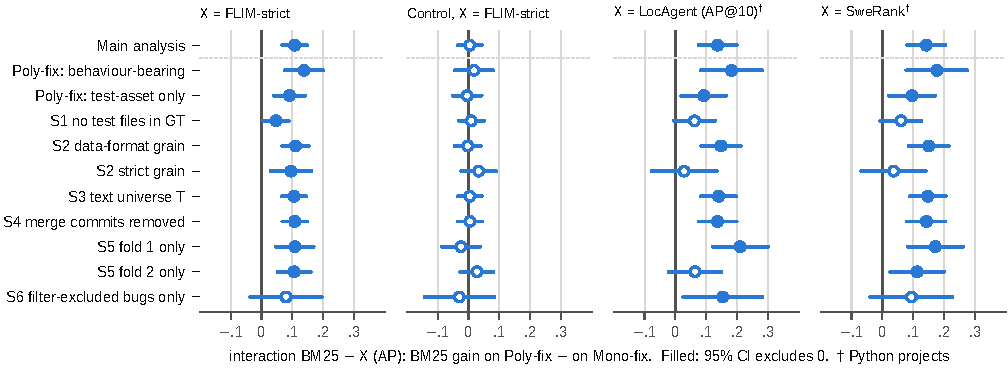
\includegraphics[width=\textwidth]{figures/fig_sensitivity.pdf}
\caption{RQ4 interaction (BM25's gain over technique X on Poly-fix bugs minus its gain on Mono-fix bugs, AP) under each sensitivity condition, with 95\% confidence intervals. The control compares BM25 restricted to parseable files with FLIM-strict. The RQ3 class effects under the same conditions are in Table~\ref{tab:sens}.}
\label{fig:sens}
\end{figure*}

\section{RQ5 details}\label{app:rq5}

With its corpus extended to all text files, SweRank's retriever
ranks the secondary-language files of Poly-fix bugs at a MAP of 0.252,
against 0.001 with Python functions only and 0.226 for BM25 on the same bugs
(paired difference $+0.026$, 90\% interval $[-0.012, 0.065]$). Its reranker,
trained on Python functions alone, keeps them there (0.257; $+0.031$
$[-0.008, 0.070]$). Neither is shown to be better than BM25, but both are
non-inferior within 0.03 (one-sided $p = 0.006$ and $0.004$). For test assets
(184 bugs) the same holds (full SweRank 0.238 against 0.208, non-inferior,
$p = 0.016$). For behaviour-bearing files (66 bugs) the data cannot tell:
full SweRank reaches 0.290 against 0.278 for BM25, with an interval from
$-0.067$ to $+0.086$, and the retriever alone 0.220 ($-0.058$
$[-0.118, 0.001]$). Because SweRank also ranks the Python files better, the
whole ranking improves: MAP over all bugs rises from 0.408 to 0.546
($+0.138$ $[0.121, 0.155]$), by 0.106 on Mono-fix and 0.198 on Poly-fix bugs
(interaction $+0.126$ $[0.084, 0.168]$). The adjusted class effect falls by
about three quarters, from $-0.172$ to $-0.044$ $[-0.102, 0.013]$; a penalty of
up to 0.10 remains compatible with the data (equivalence within $\pm0.05$:
$p = 0.43$), and for the retriever alone the class effect is still
significant ($-0.063$ $[-0.121, -0.005]$). Without test files in the ground
truth the estimate is $+0.002$. SweRank on all files outperforms BM25
on both classes (by 0.219 and 0.156), and its interaction with BM25 is
indistinguishable from 0 ($+0.015$ $[-0.042, 0.072]$; fractional logit
$p = 0.92$).

The three partial corpora separate the files that the extension adds.
Run through the full technique, adding only the non-Python files gives an
interaction of $+0.153$ $[0.131, 0.176]$ against SweRank as published:
Poly-fix MAP rises by 0.120 $[0.099, 0.142]$ (0.277 to 0.397), and Mono-fix
MAP falls by 0.015 $[0.007, 0.023]$ because the added files compete with the
fixed Python files. Part of the narrower gap therefore comes from the
Mono-fix side, as for FLIM's co-change variant below. The class effect falls
to $-0.020$ $[-0.072, 0.031]$, not significant and not shown to be negligible
(equivalence within $\pm0.05$: $p = 0.13$); without test files in the ground
truth it is $0.000$. The secondary files are ranked at a MAP of 0.261,
non-inferior to BM25 within 0.03 ($p = 0.004$), and the interaction with BM25
is indistinguishable from 0 ($-0.009$ $[-0.071, 0.053]$) while SweRank leads
in both classes. The retriever alone gives the same picture (interaction
$+0.150$ $[0.128, 0.172]$, class effect $-0.023$). Adding only the Python
test files, at the retriever, raises both classes, Mono-fix more ($+0.111$
$[0.092, 0.131]$ against $+0.062$ $[0.047, 0.078]$), because test files are
in the ground truth of many Mono-fix fixes too; the class effect widens to
$-0.207$. Adding them on top of the non-Python files in the full technique
raises Mono-fix bugs by 0.121 and Poly-fix bugs by 0.078 (interaction
$-0.028$ $[-0.065, 0.009]$). The reduction of the penalty thus comes from the
secondary-language files, which is the reach explanation of RQ2; the test
files explain why the full extension raises Mono-fix bugs as well. Capping each
file at 10 chunks instead of 40 lowers both classes slightly ($-0.015$ and
$-0.023$) and leaves the class effect at $-0.074$, so the result does not
depend on the cap.

The gap holds for behaviour-bearing
files (0.038 and 0.123 against 0.199) and for test assets (0.064 and 0.144
against 0.204).

\paragraph{A hybrid with BM25 recovers part of the loss.} Letting BM25 rank
the files a technique cannot represent raises every technique on Poly-fix
bugs: FLIM-strict by 0.051 $[0.041, 0.063]$, LocAgent by 0.096
$[0.072, 0.120]$ (AP@10) and SweRank by 0.103 $[0.080, 0.127]$ (paired
differences; every interaction with the original technique excludes 0). Over
all bugs the hybrid adds 0.054 $[0.041, 0.066]$ to LocAgent and 0.057
$[0.045, 0.068]$ to SweRank. For FLIM-strict it adds nothing
($+0.001$ $[-0.004, 0.006]$): it moves accuracy from Mono-fix bugs
($-0.021$) to Poly-fix bugs. The class effects narrow to $-0.050$,
$-0.101$ and $-0.110$. Each hybrid outperforms BM25 on Poly-fix bugs (by
0.022, 0.059 and 0.061, all intervals excluding 0). They recover less than
extending SweRank's corpus. Fusing two lists ranks the secondary files by
lexical similarity alone and interleaves them with files the technique ranks
better, so they reach a lower MAP on those files (0.128 for the SweRank
hybrid, against 0.226 for BM25 alone).

\paragraph{History instead of BM25: which is better depends on the technique.}
Ranking the missing files by how often they changed together with the
technique's top files gives Poly-fix MAPs close to the BM25 hybrid for
FLIM-strict (0.306 against 0.296; difference $+0.010$ $[-0.002, 0.022]$) and
SweRank (0.400 against 0.380; $+0.020$ $[-0.005, 0.044]$), and a lower one for
LocAgent (0.314 against 0.349; $-0.035$ $[-0.059, -0.010]$). On the secondary
files themselves the history ranks better than BM25 fusion for FLIM-strict
(0.170 against 0.140; $+0.030$ $[0.006, 0.053]$) and SweRank (0.162 against
0.128; $+0.034$ $[0.002, 0.065]$), and not significantly worse for LocAgent
(0.101 against 0.123; $-0.023$, interval $[-0.052,\allowbreak 0.005]$). Over all bugs the picture
differs again. For FLIM-strict the co-change variant costs more on Mono-fix
bugs ($-0.045$ against $-0.021$ for the hybrid), so its MAP over all bugs
falls by 0.013 $[0.007, 0.019]$ and it trails the hybrid by 0.014
$[0.008, 0.020]$. For LocAgent the hybrid is better by 0.038 $[0.023, 0.052]$,
and for SweRank the two are level ($0.000$ $[-0.015, 0.016]$). FLIM-strict's
class effect falls to $-0.025$ $[-0.065, 0.015]$; LocAgent's and SweRank's
remain ($-0.093$ and $-0.082$). Change coupling is therefore a second cheap
source for the files a parser-dependent technique cannot see, better than
lexical fusion at ranking those files for two of the three techniques but not
better over all bugs for any. Neither source reaches what SweRank achieves
when it ranks those files itself.

\section{No-primary and filter-excluded bugs}\label{app:removed}

The filter-excluded bugs were classified with the same frozen ruleset (RQ1). In
97.5\% of the filter-excluded reports that our rule would keep, our matcher finds a counted fix file
named in the title or body; for the Poly-fix ones the named file is a
primary-language file in 77.4\% and a secondary-language file in 20.8\% of
reports. 202 filter-excluded bugs fall into the fold-1 test periods (34 Poly-fix) and
235 into the fold-2 test periods (34 Poly-fix). They are scored by every
technique with the model trained on the primary-anchored bugs; none is used for training.
They are analysed as a separate group and never pooled with the primary-anchored bugs in
the main results.

On these 432 bugs (364 Mono-fix, 68 Poly-fix) every technique scores higher
than on the primary-anchored bugs, but FLIM gains most: on Mono-fix bugs its MAP is 0.496
against 0.374 for BM25, a lead twice as large as on the primary-anchored bugs. The filter
therefore did not remove the bugs on which classical retrieval is
comparatively strongest. On the Poly-fix filter-excluded bugs BM25 again exceeds
FLIM-strict (0.352 against 0.292); the interaction ($+0.080$) has the sign of
the main result but, with 68 Poly-fix bugs, an interval that includes 0
$[-0.036, 0.195]$. The same holds for SweRank on the filter-excluded bugs of the
Python projects ($+0.095$ $[-0.039, 0.228]$), while LocAgent's interaction
excludes 0 there ($+0.154$).

The 287 no-primary fixes in the test periods are the extreme case: no
ground-truth file is in the primary language, so FLIM and LocAgent can reach
none of their ground-truth files. For BM25, 98.6\% of them have a reachable
ground-truth file, and its MAP is 0.165. BLAZE, which reads every file, was
scored on them with the models trained on the primary-anchored bugs: its MAP
is 0.091, below BM25 by 0.074 $[0.038, 0.109]$. Counting them changes the
overall comparison: over the primary-anchored and no-primary test bugs of all
six projects, FLIM-strict and BM25 are level (MAP 0.276 and 0.277;
difference $-0.001$ $[-0.016, 0.015]$, equivalent within $\pm0.03$, TOST
$p<0.001$), whereas over the primary-anchored bugs alone FLIM-strict leads
(0.332 against 0.300). The change is concentrated where no-primary bugs are
common: FLIM-strict falls from 0.298 to 0.190 in dolphinscheduler (156
no-primary test bugs), by 0.040 and 0.048 in elasticsearch and airflow (55
and 51), and by at most 0.029 in the three projects with ten or fewer. One hundred of
dolphinscheduler's no-primary test bugs are fixes of its TypeScript and Vue
front-end, which a Java benchmark would usually leave out; without them
FLIM-strict leads by 0.011 $[-0.006, 0.027]$, still equivalent within
$\pm0.03$ ($p=0.009$). On the Python projects SweRank still leads BM25 (0.378
against 0.340), by less than on the primary-anchored bugs (0.408 against
0.349).

\section{Run-to-run variation and contamination}\label{app:runs}

BLAZE ranks below BM25 in both classes (MAP 0.255
and 0.244). Its published configuration fine-tunes on about 11{,}000 bugs
pooled across projects; our within-project training sets have 68--607, and
the cross-project setting is outside this study. Because BLAZE is weak in both
classes, its small class effect could partly be a floor effect; the claim that
reading every file avoids the penalty rests mainly on BM25. Across seeds, MAP varies by an
SD of 0.012--0.030 (Table~\ref{tab:seeds}), a fifth or less of the class
effects above. LocAgent's AP@10 varies by an SD of 0.009--0.022 over three runs,
and its Top-10 outcome is the same in all runs for 92.8\% of the repeated
bugs. SweRank's re-run reorders the functions of 20 of 21 bugs and the top
ten files of 12, but changes per-bug AP by 0.002 on average (at most 0.042), leaves
the Top-10 outcome of every bug unchanged and gives a MAP of 0.567 against
0.569.

The learning rate
was selected on a small validation set for some projects (8--10 bugs for
liquibase), and BLAZE's selected run reached the 15-epoch limit in two of
twelve project--folds (Table~\ref{tab:lr}). Training randomness is measured
with three seeds on three projects only; the seed SD (0.012--0.030 MAP) is
small against the effects reported, but was not measured on the other three
projects. LocAgent samples at temperature 1.0 and was run once per bug, with
two repeats on a subset (Table~\ref{tab:seeds}).

In a closed-book probe, the
LocAgent model was given only the repository name and the issue title, without
repository access, and asked which files the fix changed. Over the test bugs
of all three Python projects it named a correct file among ten for 7.1\% and
6.6\% of the Mono-fix bugs of folds~1 and~2 and for 3.3\% and 0.8\% of the
Poly-fix bugs, against 82\% Top-10 for LocAgent with repository access.
The probe is asymmetric: the model names Mono-fix files more often than
Poly-fix files, so memorisation, small as it is, favours Mono-fix bugs and
could slightly inflate the interaction. SweRank's models rank code they are
shown and cannot be probed this way, and a date-based check is not possible:
every test bug (the latest reported in March 2024) predates the release of
every model we use (SweRankEmbed's base encoder in April 2024, Qwen2.5-Coder,
on which SweRankLLM and the LocAgent model are built, in late 2024). SweRank's training data was mined from popular Python repositories,
excluding those in SWE-bench and LocBench; ansible is in LocBench and so was
excluded, but airflow and localstack may have been included, and the training
set is not released, so we cannot check. The reach result of RQ5 is less
exposed to this threat: SweRank's models were fine-tuned to rank Python
functions only, so its ranking of the YAML, JSON and other non-Python files
in the all-text variant cannot come from memorised fine-tuning targets; only
the base models' general pretraining remains as a possible source.

% generated by Scripts/analysis/paper_tables.py -- do not edit
\begin{table}[t]
\caption{Run-to-run variation, fold 1: mean $\pm$ SD over seeds 13, 42 and 2027 for the neural techniques, over LocAgent's main run and its repeats on a fixed random subset of 100 test bugs (AP@10, Top-10), and SweRank's main run and a re-run on a random subset of fold-1 bugs (MAP).}
\label{tab:seeds}
\footnotesize
\setlength{\tabcolsep}{3pt}
\begin{adjustbox}{max width=\linewidth}\begin{tabular}{llrll}
\toprule
Project & Technique & Runs & MAP & MRR \\
\midrule
liquibase (J) & FLIM-strict & 3 & .305 $\pm$ .017 & .446 $\pm$ .019 \\
 & FLIM-fallback & 3 & .306 $\pm$ .018 & .445 $\pm$ .019 \\
 & BLAZE & 3 & .244 $\pm$ .014 & .398 $\pm$ .014 \\
dolphinscheduler (J) & FLIM-strict & 3 & .347 $\pm$ .027 & .462 $\pm$ .036 \\
 & FLIM-fallback & 3 & .345 $\pm$ .030 & .460 $\pm$ .040 \\
 & BLAZE & 3 & .244 $\pm$ .012 & .319 $\pm$ .020 \\
localstack (P) & FLIM-strict & 3 & .359 $\pm$ .015 & .630 $\pm$ .020 \\
 & FLIM-fallback & 3 & .390 $\pm$ .016 & .617 $\pm$ .041 \\
 & BLAZE & 3 & .284 $\pm$ .012 & .426 $\pm$ .016 \\
\midrule
ansible (P) & LocAgent (25 bugs) & 3 & .676 $\pm$ .009 & Top-10 .960 $\pm$ .000 \\
airflow (P) & LocAgent (55 bugs) & 3 & .422 $\pm$ .016 & Top-10 .836 $\pm$ .018 \\
localstack (P) & LocAgent (17 bugs) & 3 & .266 $\pm$ .022 & Top-10 .784 $\pm$ .034 \\
Python (P) & SweRank (21 bugs) & 2 & .569 / .567 & Top-10 identical 21/21 \\
\bottomrule
\end{tabular}\end{adjustbox}
\\[2pt]{\footnotesize LocAgent: the Top-10 outcome is identical across all runs for 92.8\% of the subset bugs. SweRank: main run / re-run; per-bug $|\Delta\mathrm{AP}|$ mean .002, max .042; the function order is identical for 1 of 21 bugs.}
\end{table}



\end{document}
